%  LaTeX support: latex@mdpi.com 
%  In case you need support, please attach all files that are necessary for compiling as well as the log file, and specify the details of your LaTeX setup (which operating system and LaTeX version / tools you are using).

%=================================================================
%\documentclass[preprints,article,accept,moreauthors,pdftex]{Definitions/mdpi} 
\documentclass[aerospace,article,submit,moreauthors,pdftex]{Definitions/mdpi} 

% If you would like to post an early version of this manuscript as a preprint, you may use preprint as the journal and change 'submit' to 'accept'. The document class line would be, e.g., \documentclass[preprints,article,accept,moreauthors,pdftex]{mdpi}. This is especially recommended for submission to arXiv, where line numbers should be removed before posting. For preprints.org, the editorial staff will make this change immediately prior to posting.

%%%%%%%%%%%%%%%%%%%%%%%%%%%%%%%%%%%%%%%%%%%%%%%%%%%%%%%%%%
%% additional packages
\usepackage[printonlyused]{acronym}
\usepackage{comment}
% avoid acronym links
\makeatletter
\AtBeginDocument{%
  \renewcommand*{\AC@hyperlink}[2]{%
    \begingroup
      \hypersetup{hidelinks}%
      \hyperlink{#1}{#2}%
    \endgroup
  }%
}
\makeatother

% acrolist line spacing
\usepackage{xpatch}
\makeatletter
\xpatchcmd{\AC@deflist}
  {\addtolength{\leftmargin}{\labelsep}}
  {\addtolength{\leftmargin}{\labelsep}\setlength{\itemsep}{10pt}}
  {}{}
\makeatother

% comments
\newcommand{\Jakob}[1]{{{\color{orange}{\itshape{#1}}\color{black}}
    }{\ignorespaces}}
    
% subfigures
\usepackage{caption}
\usepackage{subcaption}

% revision highlights
\newcommand{\revision}[1]{{{\color{ForestGreen}{{#1}}\color{black}}
    }{\ignorespaces}}
%\newcommand{\revision}[1]{\color{green}{#1 }\color{black}}
%%%%%%%%%%%%%%%%%%%%%%%%%%%%%%%%%%%%%%%%%%%%%%%%%%%%%%%%%%


%--------------------
% Class Options:
%--------------------
%----------
% journal
%----------
% Choose between the following MDPI journals:
% acoustics, actuators, addictions, admsci, aerospace, agriculture, agriengineering, agronomy, algorithms, animals, antibiotics, antibodies, antioxidants, applsci, arts, asc, asi, atmosphere, atoms, axioms, batteries, bdcc, behavsci , beverages, bioengineering, biology, biomedicines, biomimetics, biomolecules, biosensors, brainsci , buildings, cancers, carbon , catalysts, cells, ceramics, challenges, chemengineering, chemistry, chemosensors, children, cleantechnol, climate, clockssleep, cmd, coatings, colloids, computation, computers, condensedmatter, cosmetics, cryptography, crystals, dairy, data, dentistry, designs , diagnostics, diseases, diversity, drones, econometrics, economies, education, ejihpe, electrochem, electronics, energies, entropy, environments, epigenomes, est, fermentation, fibers, fire, fishes, fluids, foods, forecasting, forests, fractalfract, futureinternet, futurephys, galaxies, games, gastrointestdisord, gels, genealogy, genes, geohazards, geosciences, geriatrics, hazardousmatters, healthcare, heritage, highthroughput, horticulturae, humanities, hydrology, ijerph, ijfs, ijgi, ijms, ijns, ijtpp, informatics, information, infrastructures, inorganics, insects, instruments, inventions, iot, j, jcdd, jcm, jcp, jcs, jdb, jfb, jfmk, jimaging, jintelligence, jlpea, jmmp, jmse, jnt, jof, joitmc, jpm, jrfm, jsan, land, languages, laws, life, literature, logistics, lubricants, machines, magnetochemistry, make, marinedrugs, materials, mathematics, mca, medicina, medicines, medsci, membranes, metabolites, metals, microarrays, micromachines, microorganisms, minerals, modelling, molbank, molecules, mps, mti, nanomaterials, ncrna, neuroglia, nitrogen, notspecified, nutrients, ohbm, optics, particles, pathogens, pharmaceuticals, pharmaceutics, pharmacy, philosophies, photonics, physics, plants, plasma, polymers, polysaccharides, preprints , proceedings, processes, proteomes, psych, publications, quantumrep, quaternary, qubs, reactions, recycling, religions, remotesensing, reports, resources, risks, robotics, safety, sci, scipharm, sensors, separations, sexes, signals, sinusitis, smartcities, sna, societies, socsci, soilsystems, sports, standards, stats, surfaces, surgeries, sustainability, symmetry, systems, technologies, test, toxics, toxins, tropicalmed, universe, urbansci, vaccines, vehicles, vetsci, vibration, viruses, vision, water, wem, wevj

%---------
% article
%---------
% The default type of manuscript is "article", but can be replaced by: 
% abstract, addendum, article, benchmark, book, bookreview, briefreport, casereport, changes, comment, commentary, communication, conceptpaper, conferenceproceedings, correction, conferencereport, expressionofconcern, extendedabstract, meetingreport, creative, datadescriptor, discussion, editorial, essay, erratum, hypothesis, interestingimages, letter, meetingreport, newbookreceived, obituary, opinion, projectreport, reply, retraction, review, perspective, protocol, shortnote, supfile, technicalnote, viewpoint
% supfile = supplementary materials

%----------
% submit
%----------
% The class option "submit" will be changed to "accept" by the Editorial Office when the paper is accepted. This will only make changes to the frontpage (e.g., the logo of the journal will get visible), the headings, and the copyright information. Also, line numbering will be removed. Journal info and pagination for accepted papers will also be assigned by the Editorial Office.

%------------------
% moreauthors
%------------------
% If there is only one author the class option oneauthor should be used. Otherwise use the class option moreauthors.

%---------
% pdftex
%---------
% The option pdftex is for use with pdfLaTeX. If eps figures are used, remove the option pdftex and use LaTeX and dvi2pdf.

%=================================================================
\firstpage{1} 
\makeatletter 
\setcounter{page}{\@firstpage} 
\makeatother
\pubvolume{xx}
\issuenum{1}
\articlenumber{5}
\pubyear{2019}
\copyrightyear{2019}
%\externaleditor{Academic Editor: name}
\history{Received: date; Accepted: date; Published: date}
%\updates{yes} % If there is an update available, un-comment this line

%% MDPI internal command: uncomment if new journal that already uses continuous page numbers 
%\continuouspages{yes}

%------------------------------------------------------------------
% The following line should be uncommented if the LaTeX file is uploaded to arXiv.org
%\pdfoutput=1

%=================================================================
% Add packages and commands here. The following packages are loaded in our class file: fontenc, calc, indentfirst, fancyhdr, graphicx, lastpage, ifthen, lineno, float, amsmath, setspace, enumitem, mathpazo, booktabs, titlesec, etoolbox, amsthm, hyphenat, natbib, hyperref, footmisc, geometry, caption, url, mdframed, tabto, soul, multirow, microtype, tikz

%=================================================================
%% Please use the following mathematics environments: Theorem, Lemma, Corollary, Proposition, Characterization, Property, Problem, Example, ExamplesandDefinitions, Hypothesis, Remark, Definition, Notation, Assumption
%% For proofs, please use the proof environment (the amsthm package is loaded by the MDPI class).

%=================================================================
% Full title of the paper (Capitalized)
\Title{Design Space Exploration of a Jet Engine Component using a Combined Object Model for Function and Geometry}

% Author Orchid ID: enter ID or remove command
\newcommand{\orcidauthorA}{0000-0002-2270-6253} % Add \orcidA{} behind the author's name
\newcommand{\orcidauthorB}{0000-0001-5216-0944} % Add \orcidB{} behind the author's name
\newcommand{\orcidauthorC}{0000-0003-0373-3720} % Add \orcidC{} behind the author's name

% Authors, for the paper (add full first names)
\Author{Jakob R. Müller $^{1}$*\orcidA{}, Massimo Panarotto $^{1}$\orcidB{} and Ola Isaksson $^{1,}$\orcidC{}}

% Authors, for metadata in PDF
\AuthorNames{Jakob R. Müller, Massimo Panarotto and Ola Isaksson}

% Affiliations / Addresses (Add [1] after \address if there is only one affiliation.)
\address{%
$^{1}$ \quad Chalmers University of Technology, Gothenburg}

% Contact information of the corresponding author
\corres{Correspondence: jakob.muller@chalmers.se}

% Current address and/or shared authorship
%\firstnote{Current address: Affiliation 3} 
%\secondnote{These authors contributed equally to this work.}
% The commands \thirdnote{} till \eighthnote{} are available for further notes

%\simplesumm{} % Simple summary

%\conference{} % An extended version of a conference paper

% Abstract (Do not insert blank lines, i.e. \\) 
\abstract{The design of aircraft and engine components hinges on the use of CAD models and the subsequent geometry-based analyses for evaluation of the quality of a concept.
However, the generation (and variation) of a CAD models to include radical or novel design solutions is a resource intense modelling effort.
While approaches to automate the generation and variation of CAD models exist, they do neglect the capture and representation of the product's design rationale---what the product is supposed to do.
The design space exploration approach Function and Geometry Exploration (FGE) aims to support the exploration of more functionally and geometrically different product concepts under consideration of not only geometrical, but also teleological aspects.
The FGE approach has been presented and verified in a previous presentation.
However, in order to contribute to engineering design practice, a design method needs to be validated through application in industrial practice.
%A novel method for associative Function and Geometry Exploration (FGE) has been applied and first validated in a conceptual design study of a Guide Vane (GV) of a turbofan engine. 
Hence, this publication reports from a study where the FGE approach has been applied 
%The FGE method and its software tool implementation were introduced and used
by a design team of a Swedish aerospace manufacturer in a conceptual product development project.
Conceptually different alternatives where identified in order to meet the expected functionality of a guide vane (GV).
The FGE was introduced and applied in a series of workshops.
Data was collected through participatory observation in the design teams by the researchers as well as interviews and questionnaires.
%The applicability and validity of FGE as a design method was in addition evaluated using interviewing the design team participants and through questionnaires. 
The results reveal the  potential of the FGE approach as a design support to:
1) represent and capture the design rationale and the design space
2) capture, integrate and model novel solutions and 
3) provide support for the embodiment of novel concepts that would otherwise remain unexplored.
In conclusion, the FGE method supports designers to articulate and link the design rationale, including functional requirements and alternative solutions, to geometrical features of the product concepts.
The method supports the exploration of alternative solutions as well as functions. 
%The FGE tool, which is still in a laboratory state, required facilitation by researchers, yet showed to be sufficiently capable of generating and representing the alternatives studied in real time.
However, scalability and robustness of the generated CAD models remain subject to further research.
}
%% Reset all acronyms for main part:
% Keywords
\keyword{Product development process, Design space exploration, Function modelling, CAD, Aerospace}

% The fields PACS, MSC, and JEL may be left empty or commented out if not applicable
%\PACS{J0101}
%\MSC{}
%\JEL{}

%%%%%%%%%%%%%%%%%%%%%%%%%%%%%%%%%%%%%%%%%%
% Only for the journal Diversity
%\LSID{\url{http://}}

%%%%%%%%%%%%%%%%%%%%%%%%%%%%%%%%%%%%%%%%%%
% Only for the journal Applied Sciences:
%\featuredapplication{Authors are encouraged to provide a concise description of the specific application or a potential application of the work. This section is not mandatory.}
%%%%%%%%%%%%%%%%%%%%%%%%%%%%%%%%%%%%%%%%%%

%%%%%%%%%%%%%%%%%%%%%%%%%%%%%%%%%%%%%%%%%%
% Only for the journal Data:
%\dataset{DOI number or link to the deposited data set in cases where the data set is published or set to be published separately. If the data set is submitted and will be published as a supplement to this paper in the journal Data, this field will be filled by the editors of the journal. In this case, please make sure to submit the data set as a supplement when entering your manuscript into our manuscript editorial system.}

%\datasetlicense{license under which the data set is made available (CC0, CC-BY, CC-BY-SA, CC-BY-NC, etc.)}

%%%%%%%%%%%%%%%%%%%%%%%%%%%%%%%%%%%%%%%%%%
% Only for the journal Toxins
%\keycontribution{The breakthroughs or highlights of the manuscript. Authors can write one or two sentences to describe the most important part of the paper.}

%\setcounter{secnumdepth}{4}
%%%%%%%%%%%%%%%%%%%%%%%%%%%%%%%%%%%%%%%%%%
\begin{document}
%%%%%%%%%%%%%%%%%%%%%%%%%%%%%%%%%%%%%%%%%%

%\acresetall
% %%%%%%%%%%%%%%%%%%%%%%%%%%%%%%%%%%%%%%%%%%
% \setcounter{section}{-1} %% Remove this when starting to work on the template.
% \section{How to Use this Template}
% The template details the sections that can be used in a manuscript. Note that the order and names of article sections may differ from the requirements of the journal (e.g., the positioning of the Materials and Methods section). Please check the instructions for authors page of the journal to verify the correct order and names. For any questions, please contact the editorial office of the journal or support@mdpi.com. For LaTeX related questions please contact latex@mdpi.com.
% %The order of the section titles is: Introduction, Materials and Methods, Results, Discussion, Conclusions for these journals: aerospace,algorithms,antibodies,antioxidants,atmosphere,axioms,biomedicines,carbon,crystals,designs,diagnostics,environments,fermentation,fluids,forests,fractalfract,informatics,information,inventions,jfmk,jrfm,lubricants,neonatalscreening,neuroglia,particles,pharmaceutics,polymers,processes,technologies,viruses,vision

\section{Introduction}


% Points to make in intro:
% This is a VALIDATION STUDY which is something that needs to be done in EDR, as stated by:
% \cite{Gero2016} "testing research claim"
% However, this appears to be difficult, to the point that "a majority of papers in the field do not explicitly address validation" \citep{Barth2011}.
% findings from a complex, real-life development project are very difficult, or meaningless, to prove in a mathematical manner" \citep{Almefelt2006} therefore real life experiments needed, such as this one here
% method needs to be "useful[..] in respect to a purpose" \citep{Barlas1990}.
% methods and tools that are developed in the course of \ac{EDR} to be powerful, reliable and validated \citep{Eckert2003}

%FGE has been presented in \cite{Muller2020a}: this is just a study of its application!
%still a quick recap;

The development of new components for aircraft engines often relies on an improvement and refinement of an existing "legacy design".
To be able to meet the targets set by Flightpath 2050 \cite{ACARE2017StrategicAgenda}, \revision{as well as contemporary developments in air travel \citep{Schmidt2020Commercial2020},} manufacturers need to explore and develop conceptually new designs.
Such novel concepts are required on aircraft and engine system level, but equally on component level \cite{Filipenko2020ComparativeSystems, Parker2010GreenEnvironment}.

\revision{
Examples for such novel product concepts are the open rotor design \cite{Larsson2006ComponentInnovation} or electrical and hybrid propulsion designs \citep{Dale2020ElectricPropulsion}.
Such concepts bring new arrangements and require new functions to be met by the engine components.}
 
Such radically new concepts---as well as the components they are composed of---need to be \revision{developed, designed and} evaluated first.
In the case of developing physical products,\revision{ such as aeroengine components, this} requires their embodiment in a sufficient level of \revision{detail} for engineering analysis.
\revision{In most cases, }this means that a geometry model\revision{ in the form of \ac{CAD} }of each concept \revision{needs to be created. 
To be able to assess all relevant product properties, analyses on \textit{solid models} may be required \citep{Hirz2013}.
As a result, this publication is focused on the management and generation of solid CAD models.}

%Also, manufactures are interested to introduce new functions in their products in order to maintain competitiveness in the market. 

% need for DSE
To be able to develop novel products outside the already known design space, developers need reliable methods and tools that support them in the generation of concepts and models as well as their analysis and evaluation \cite{Woodbury2006, Kang2011, Isaksson2016}.
% currently available tools insufficient
Currently available -- and applied -- methods such as parameterisation \citep{VanDerLaan2005ParametricAnalysis} or \ac{KBE} \cite{Sandberg2011} cover only a dimensional variation of existing concepts or require an expensive setup of a master model.
Therefore, these geometry based approaches only allow for the exploration of a subset of the available design space \citep{Woodbury2006, Muller2019ICED}.
\revision{To enable conceptual design which explores alternative functions and solutions, a \ac{DSE} method needs to take into account a representation of the product's \textit{function} \citep{Umeda1997FunctionalDesign, Cohrs2014}.

The \ac{DSE} method \textit{\acf{FGE}} has been developed to fulfil this premise: through a connection of the functional and geometrical domain, a wider and more efficient exploration is to be enabled \citep{Muller2021FunctionVariants}.
%To enable a systematic, wide and efficient \ac{DSE}, an approach connecting function and geometry models, named \textit{\ac{FGE}}, has been developed \cite{Muller2021FunctionVariants}.
%\Ac{FGE} enables the automated generation of CAD models of variant concepts based on alternative solutions captured in a function model.
%The approach enables product developers to associate the geometry directly with the function it fulfils and vice versa; thereby FGE aims to enable a parallel development approach in both, the functional and geometrical, domains.
However, while the \ac{FGE} approach itself has been presented and verified in \cite{Muller2021FunctionVariants}, its effect on improving \ac{DSE} in practice has not been validated.
This publication reports from a study to \textit{validate} the approach through application in an industrial setting.
Validation refers in this case to test whether it \textit{useful}, that means it has a positive impact on the product development process, in an \textit{applied context} \citep{Pedersen2000, Eckert2003Spiral}.

% Therefore, new solutions can be integrated for specific functional requirements, while allowing to only alter the related geometry and observing the impact of the alteration onto the product as a system.
% Furthermore does the approach allow to trace changes in requirements and functions onto the product's geometry, enabling a more precise redesign process in the case of requirement changes.

% paper overview
The validation is performed through a} qualitative study about the application of the \ac{FGE} approach in a development project for a static turbine structure, a fan frame \acf{GV}. 
The study has been conducted in tight collaboration with an aerospace manufacturer. 
The study investigates into whether \ac{FGE} does \textit{improve \ac{DSE}} in that it enables the \textit{capture}, \textit{representation} and \textit{embodiment} of novel design concepts.

%Section \ref{sec:background} explains the relevant technologies which the approach is build or that are comparable in functionality.

An over view over the underlying theories is given in Section \ref{sec:background}, and the \ac{FGE} approach itself is shortly explained in Section \ref{sec:omfgDSE}.
How the study has been setup and how the approach has been evaluated is explained in Section \ref{sec:method}.
The application of \ac{FGE} in the industrial setting is presented in Section \ref{sec:results}. 
The practitioners' evaluation and reflections on the application of the approach on the industrial use case  are presented in Section \ref{sec:feedback}.
Section \ref{sec:discussion} discusses these results in relation to the problematic described above as well as compared to similar approaches.
Lastly, section \ref{sec:conclusions} summarises the contribution of this paper and proposes directions for further development of the approach.


% \Jakob{Problem: DSE is too minimal in its current form. 

% Current form = legacy design, hard focus on evolutionary development of CAD model, EWB (MDA approach for DSE), parameterisation of CAD

% proposed approach: omfgDSE

% criteria:
% }

% \subsection{Design space exploration}
% The design space is the sum of all possible concepts which fulfil the requirements \cite{Saxena2010}.
% However, the number of concepts is neigh infinite \cite{Woodbury2006}, and therefor it is not possible to explore all of them.

% To \textit{explore} means in this case to generate product concept descriptions which presumably reside inside the design space -- that is, fulfil all requirements and functions -- and analyse it for its performance.
% The analysis has two-fold aim: first, to verify whether the concept actually does fulfil all requirements, and second how well it does, to be able to compare it with other designs and chose the best available.
% The concept descriptions required for this are in most cases -- especially in the aerospace industry -- CAD models \cite{}.
% These models are used for subsequent product behaviour analysis such as aerodynamic, structural or thermodynamic simulations.

% In most cases, the design space is explored by varying an existing \textit{legacy model}, and generating variants of it \cite{Prasad2006}.
% This approach, mainly building on engineers' experience and 

% \subsection{Function modelling}

% \Jakob{
% KBE: \citep{LaRocca2012}; parametric design \citep{vanderlaan2005}

% FBS \citep{Gero2004}; 

% EF-M \citep{Schachinger2000}, 

% geometric feature based modelling \citep{}, 

% }
 
\revision{
\section{Frame of reference}\label{sec:background}
%DSE general
In the conceptual phases of product development, multiple alternative concepts need to be evaluated.
The sum of all possible concepts which fulfil the respective requirements is called the \textit{design space} \citep{Saxena2010}.
The more, and more different, concepts can be investigated, which would correspond to a larger area of the design space being covered, the higher the probability that a good or even the best possible concept has been selected \citep{Woodbury2006}.

To achieve this, the design space needs to be defined, the concepts residing in it need to be devised and evaluated against each other \citep{Kang2011}.
For the evaluation against each other, that is assessing whether, and how well, they fulfil requirements and functions, the concepts' need to be simulated in terms of different behaviour. 
For most of such simulations, a geometrical product representation in the form of a \ac{CAD} model is needed \citep{Isaksson2016}.
\\

%%% geometry DSE
\Ac{CAD} models are a representation of a product's \textit{geometry} and \textit{topology}.
Geometry refers to the shape of the product, whereas topology refers to the relations to the individual shapes towards each other \citep{Gonzalez-Lluch2017ATools}. 
Most commercial CAD software operate as \textit{feature-based parametric CAD}, where geometric and topological information is contained in \textit{features} which are set into relation in a procedurally operated feature-tree.
If set-up and maintained correctly, the alteration and exchange of such features should allow for easy adjustment of the CAD model \cite{Camba2021TheRoadmap}.
Furthermore allows \textit{parameterisation} for a variation of geometry model's dimensions \cite{Camba2016a}.

% cons of CAD
While parameterised, feature-based CAD models are theoretically easily altered, in practice the alteration of is difficult.
A lack of consistent modelling practices, the complexity of relations in a master model and ambiguous feature definitions make CAD models difficult to edit and lead to failures in their regeneration \cite{Camba2021TheRoadmap, Kasik2005TenChallenges, Gonzalez-Lluch2017ATools}.
Furthermore is parameterisation considered "a big challenge", and even in the best case "offers little flexibility", since the parameterisation of the master model already defines all possible concepts and does not allow for the introduction of novel solutions \citep{Li2020AnDevelopment}.

% These shapes are in most common commercial CAD programmes created and stored as \textit{features}, containers for geometrical and topological product information.
% Such features are arranged 

% However, the creation of such parametric models is "a big challenge" \citep{Li2020AnDevelopment}.
% The creators of the model need to anticipate all possible changes of the model beforehand.
% The parameterisation needs to be performed in a way that both enables the desired changes in geometry and maintains the model's robustness.
% As a result, "a parametric model offers little flexibility" for the introduction of design solutions once the parameterisation has been performed \citep{Li2020AnDevelopment}.
% If these models are to be altered for new \ac{DS} anyway, most modelling approaches are "prone to modelling errors" \citep{Camba2016a}.


To avoid such failures, CAD models are build following design guidelines which reduce the chance for failures.
While such a composition represents the model's \textit{design intent}, this does rarely coincide with the product's \textit{\acf{DR}}.
Hence are changes to the product, which are based on the introduction of new functions or new solutions for identified functions, difficult, since the CAD model does not contain any of this teleological information \citep{Umeda1997FunctionalDesign, Cohrs2014}.
\\

%%%%%%%%%%%%%%%%%%%%%%%%%%%%%%%%%%%%%%%%%%%%%%%%%%%%%%%%%%%%%%%%%%%%
%%% function DSE
Function models on the other hand can represent a product's \ac{DR}, together with architectural or systemic product properties.
As such, they provide a good basis for teleologically motivated \ac{DSE}: through the representation of functions and solutions, developers can precisely target their design effort \citep{Levandowski2014SBCE}.
Furthermore can function models be used for systemic analysis \citep{albers2014}, automated \ac{DSE} and concept generation \citep{Helms2012, Jin2007} or product platforms \citep{landahl2018, Levandowski2014SBCE}.
However, while in some cases enabling "physics-based reasoning" \citep{Mokhtarian2017}, function models do not provide a basis for most engineering analysis, where product geometry models are needed.
Connecting the two modelling domains of function and geometry has been a long standing challenge in \ac{EDR} \citep{Umeda1997FunctionalDesign, Cohrs2014, Tomiyama2013}.
\\

% EFM
\Acf{EF-M} modelling is a function modelling approach which represents the design space through alternating \acf{FR} and \acf{DS} \cite{Schachinger2000}.
\Ac{DS} can be subject to individual constraints, which place limits on design parameters or behaviour.
The basic modelling elements of \ac{EF-M} are presented in Figure \ref{fig:EFM}.
This creates a hierarchical product architecture representation, which enables the introduction of novel solutions and sub-functions on arbitrary levels of granularity into an existing product structure \cite{Muller2020}.

%The reason for this ability of \ac{EF-M} to represent the design space through functions and constraints, capture and represent alternative solutions on any abstraction level and the option for first-level analysis based purely on a function model \cite{Muller2019Aiedam}.
%The function model is created by alternating \ac{FR} and their respective \ac{DS} in a tree like structure \cite{Schachinger2000}.
Since \ac{EF-M} follows the axiom of independence of Suh's axiomatic design \cite{Suh1990}, each \ac{FR} is---in one concept---solved by \textit{only one} \ac{DS}. 
If there are more \ac{DS} per \ac{FR} modelled, these represent alternatives.
This is illustrated in Figure \ref{fig:EFM} in the form of "Solution A" and "Solution B".

\begin{figure}[ht]
    \centering
    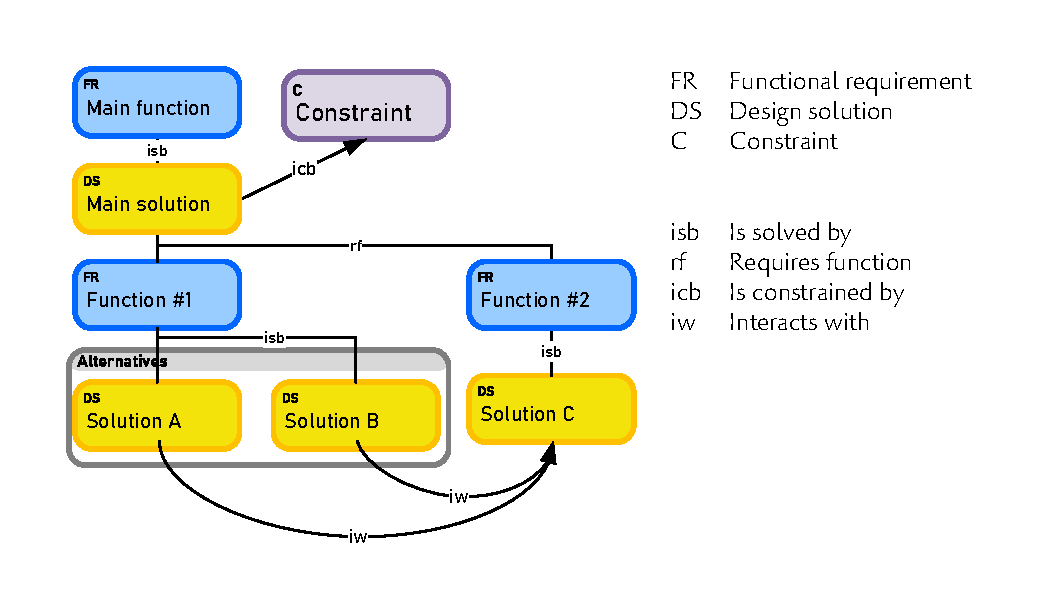
\includegraphics[width=.8\textwidth]{figures/pdf/efm_basics.pdf}    
        \caption{Enhanced Function-Means modelling elements after \cite{Schachinger2000}.}
    \label{fig:EFM}
\end{figure}

% instantiation
Since new \ac{DS} are captured for different functions on individual branches of the EF-M tree, they can be combined into a multitude of different concepts.
In the presented example in Figure \ref{fig:EFM}, only two concepts can be instantiated, one with each alternative \ac{DS}.
In Figure \ref{fig:instantiation} two times two alternatives become four concepts.
%The \textit{instantiation algorithm} that has been implemented in \ac{FGE} also manages alternatives on arbitrary sub levels of the \ac{EF-M} tree.

}


% FGE, omfg is a combination of function and geometry modelling; 
% therefore both are quickly presented here


% Originally, \acf{CAD}, the de-facto standard modelling approach for product geometry, was intended to simplify the generation of product drawings \citep{Kasik2005TenChallenges}.

% "procedural, feature based CAD" --> \citep{Gonzalez-Lluch2017ATools}

% To simplify variation of existing CAD models, \textit{parametric CAD} separates the geometric data from the governing dimensional parameters \citep{Camba2016a}.
% Beyond this, modern CAD systems also allow for the association of CAD data not only between different geometric objects, but also different modelling files \citep{Hirz2013}.
% This allows for connected assembly structures, where changes in parameters propagate through the geometry of the entire product structure.

% % challegnes


% \citep{Camba2016a} for parametric background

% \citep{Camba2021TheRoadmap} parametric challenges; need to rebuild model in case of parametric failure BUT keep DR!



% Critique: FGE allows only for investigation into certain subspace, which are not defined; 
% --> how to define them?
% counter: parameterisation allows for investigation into subspace of geometrical variation, defined through parameterisation/master model \citep{Camba2021TheRoadmap}
% This, however, introduces FURTHER subspaces which are defined through the embodiments


% \cite{Gonzalez-Lluch2017ATools} Potential errors in CAD regeneration: 
% prone to "morphological errors in procedural CAD models"  \cite{Gonzalez-Lluch2017ATools}

% NEED FOR FGE:
% \begin{itemize}
%     \item \cite{Cohrs2014} calling for "interdisciplinary integration of function architectures with CAD models", 
%     \item \cite{Tomiyama2013} highlighting the "missing direct connections with [...] geometric models" as a reason for function models being perceived as "not practical",
%     \item or \cite{Umeda1997} stating that "future CAD technology [...] should represent and reason about function".
% \end{itemize}


%%%%%%%%%%%%%%%%%%%%%%%%%%%%%%%%%%%%%%%%%%%%%%%%%%%%%%%%%%%%%%%%%%%%%%%%%%%%%%%%%%%%%%%%%%%%%%%%%%%%%%%
\subsection{The FGE approach}\label{sec:omfgDSE}
% EF-M
The \acf{FGE} approach combines the \revision{representation of product architecture and DR, and the flexibility to introduce novel solutions into an existing legacy design with a feature based CAD approach.}
The approach builds on the function modelling method \ac{EF-M} modelling and combines it with a \ac{DA} approach based on \acp{UDF}. 
One main assumption behind the approach is that every geometrical element in a product has a specific function \citep{Gero2004}.
This function can be identified, and the related geometry can be isolated.
As a result, these two information sets can be coupled. 
The other main assumption for the approach is that if the function of a geometry element is identified, alternative solutions for that function can be identified and integrated into the product architecture \cite{Levandowski2014SBCE, Muller2019Aiedam}.
\\

\begin{figure}[hb]
    \centering
    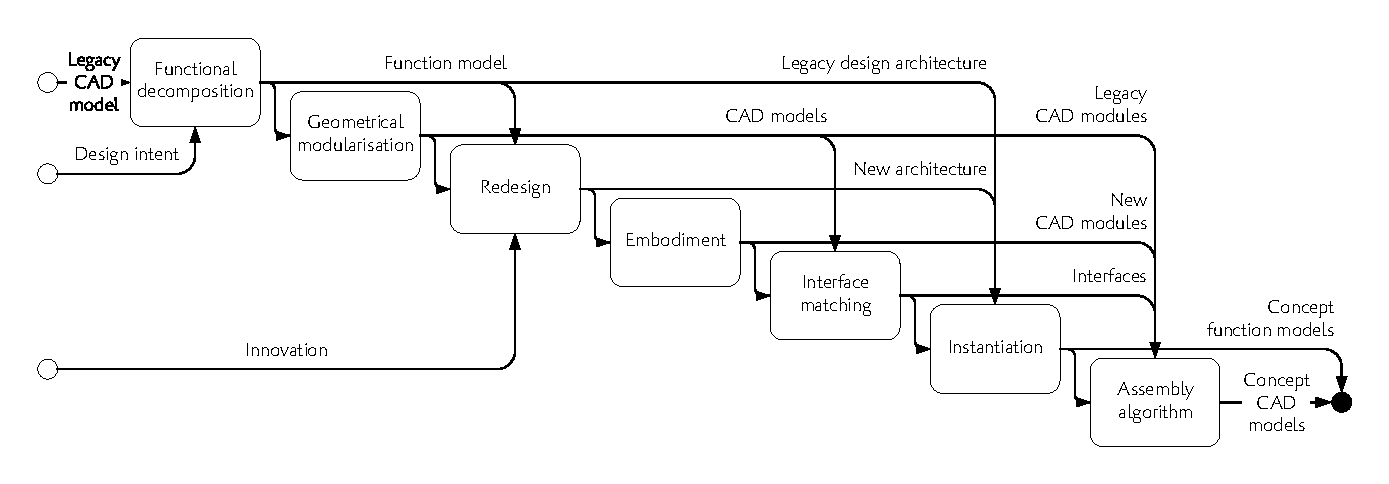
\includegraphics[width=\textwidth]{figures/pdf/FGE_IDEF0.pdf}
    \caption{IDEF0 process model of the applied FGE approach.
    }
    \label{fig:FGE_IDEF0}
\end{figure}


% base working principle: decomp, inno, embody
The \ac{FGE} method is based on three main phases: \textit{decomposition} of the legacy CAD model, an \textit{innovation} stage in the functional domain and an \textit{embodiment} phase to generate CAD models of the concepts.
\revision{Figure \ref{fig:FGE_IDEF0} presents the steps inside these three main stages:
the decomposition takes part in both the \textit{function-} as well as geometry-model, whereas the \textit{geometrical modularisation} is based on the structure of the EF-M model and the resulting UDF are directly linked to their respective DS.
The innovation stage includes \textit{redesign}, where novel functions and solutions are captured in the function model, \textit{embodiment} of said solutions into UDF and the matching of their interfaces towards the existing product structure.
Lastly, the different concepts are \textit{instantiated} first from the function model and then embodied through the included \textit{assembly algorithm}.

To represent the relations between function modelling objects and design features, the FGE approach relies on the \acf{OMFG}.
This object model has been presented and verified in \cite{Muller2021FunctionVariants}.
% Since the embodiment of all concepts has shown to be a key obstacle in investigating into multiple concepts, previous research \citep{Muller2020a} has yielded a modular CAD modelling approach that allows for the generation of CAD models of variant designs based on embodiment of only single \ac{DS}.

\begin{figure}
    \centering
    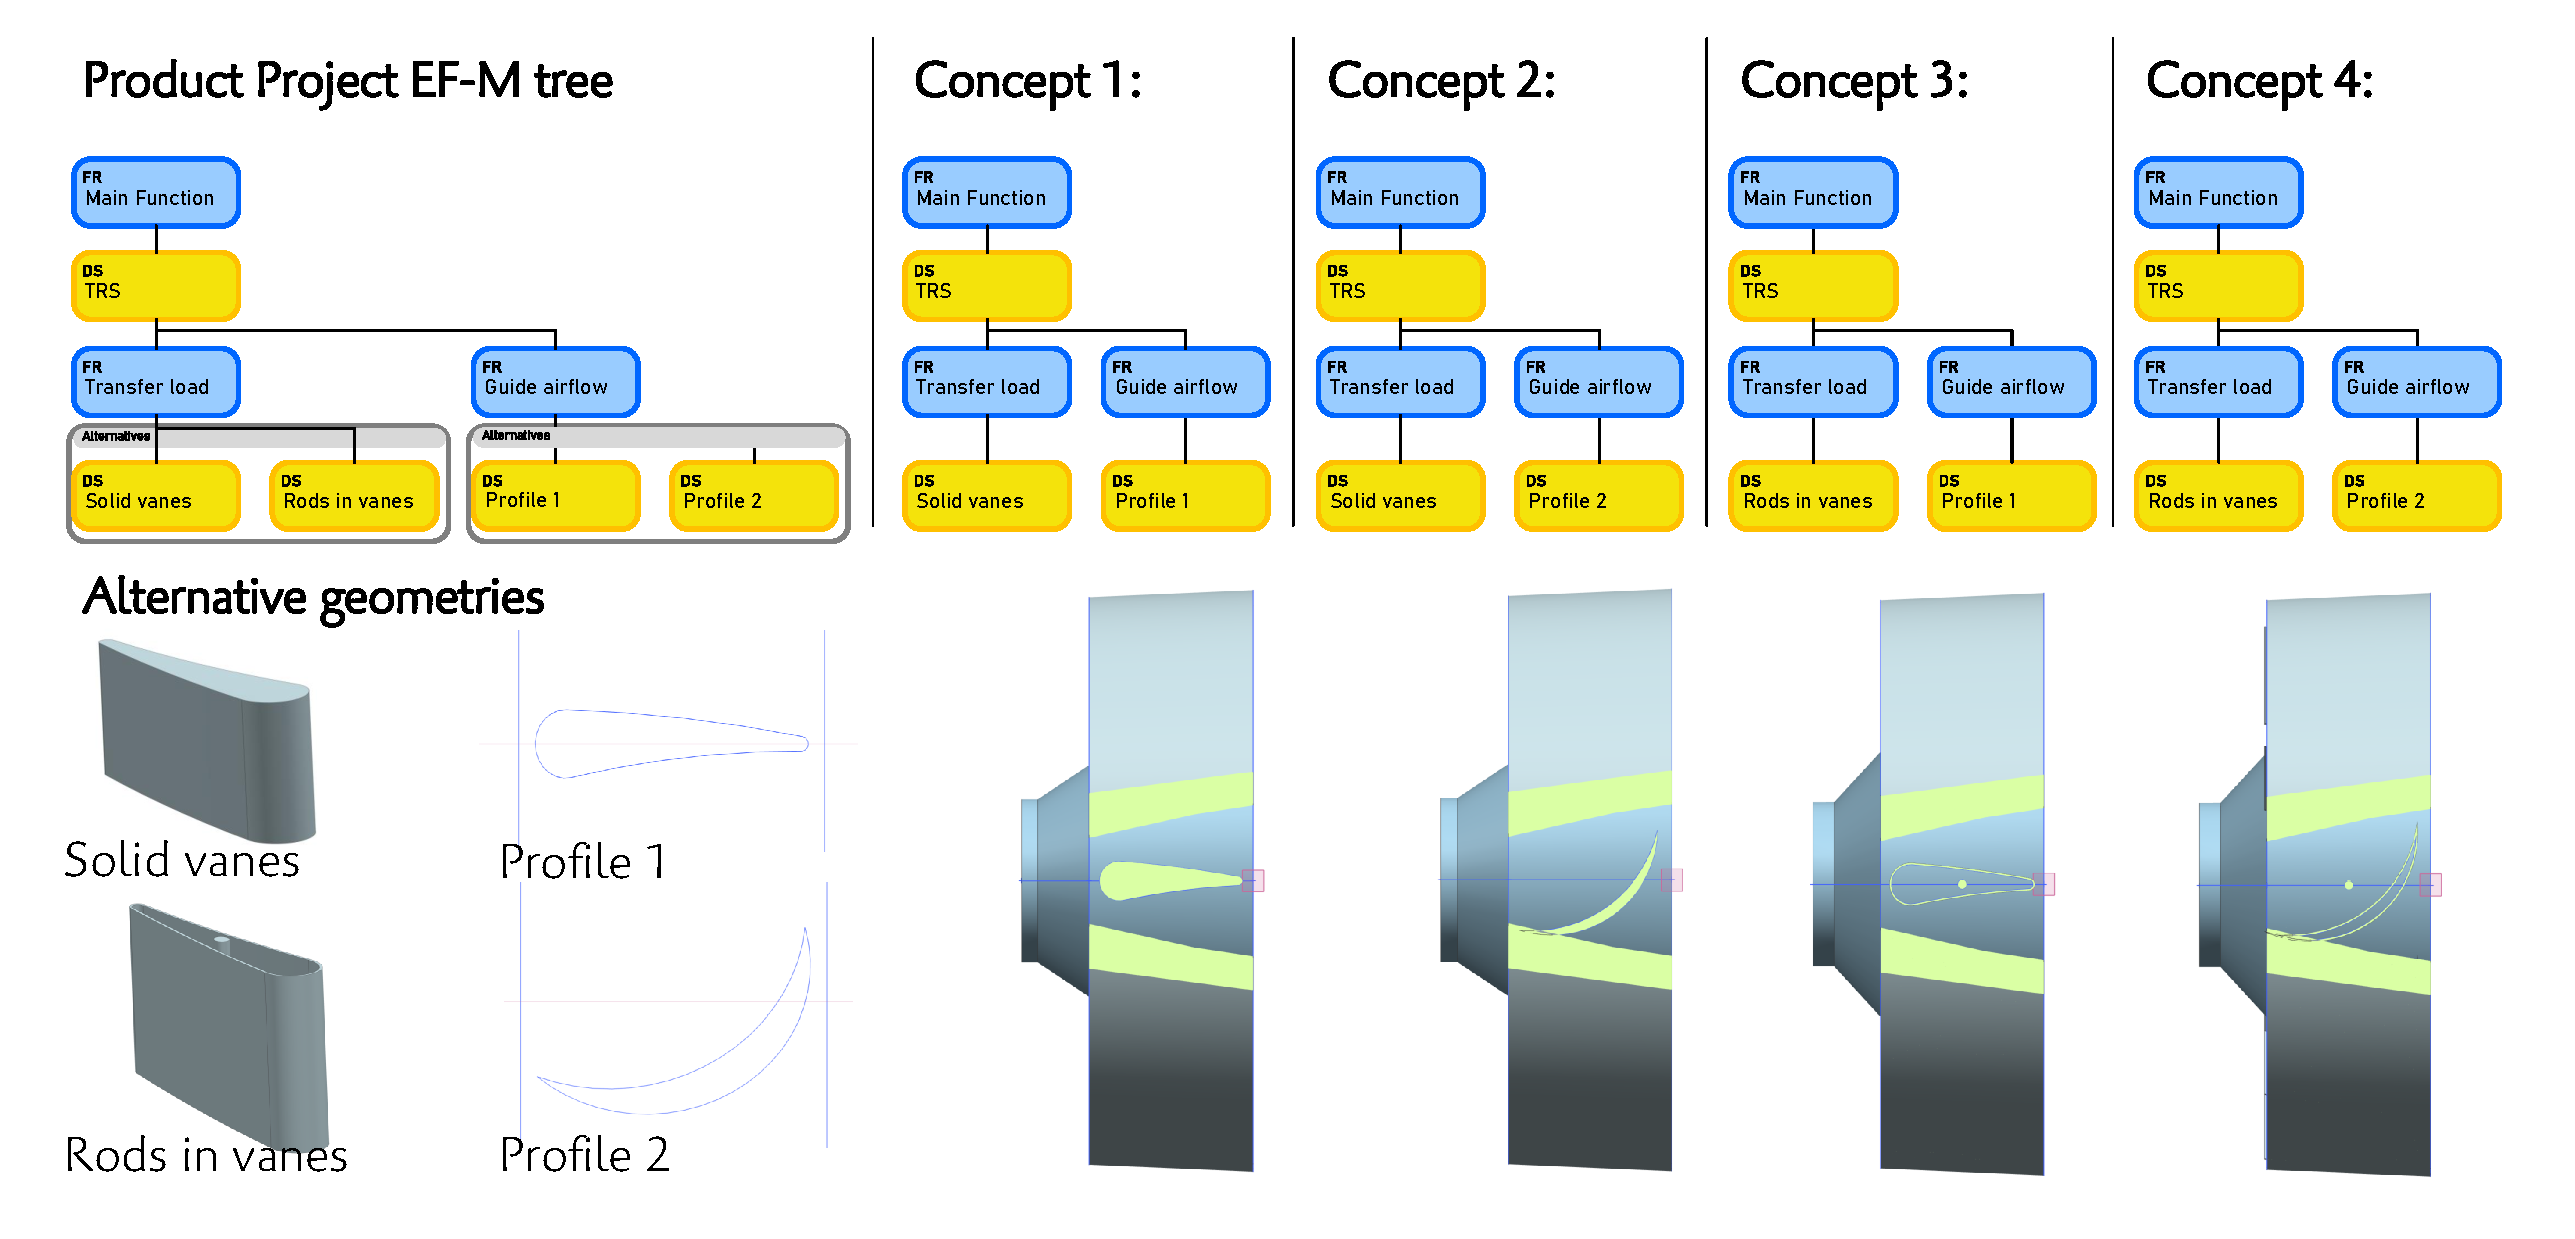
\includegraphics[width=\textwidth]{figures/pdf/instantiation.pdf}
    \caption{Instantiation in EF-M and the associated CAD model.
    Left hand side shows the EF-M model with alternative DS, and below the respectively associated UDF.
    To the right are the four resulting instances, on top in EF-M and their respective embodiment below.
    All models have been created using a proof-of-concept tool of FGE \citep{Muller2021FunctionVariants}.
    }
    \label{fig:instantiation}
\end{figure}

% DSE in FGE
The FGE approach assumes the existence of a legacy design in the form of a CAD model.
In the first step is the model is decomposed into an EF-M model, in a bottom-up approach where the functions of individual geometric elements are identified.
Once the geometrical elements are captured as DS are they linked to their function in the form of FR.
Potential constraints are also captured in the EF-M model in relation to the respective DS.
The decomposition of a legacy design into an EF-M model and the constraining of the design space in both the functional and geometrical domain is described in detail in \cite{Muller2020MappingManufacturing}.
Once they are associated to a DS, the geometrical features are captured in a \ac{UDF} with clearly defined interfaces and design parameters.
Both of these are captured in the \ac{OMFG} and provide the basis for the \ac{DA} of FGE.}

% CAD / DA / UDF
%The modularised \ac{DA} approach enables the assembly of individual CAD models for each concept based on the alternative solutions captured in the \ac{EF-M} model.
%The approach is presented in detail \cite{Muller2021FunctionVariants}.
%To enable this \ac{DA}, each \ac{DS} is coupled through the \ac{OMFG} with the \ac{UDF} embodying it.
Since \ac{UDF} are available in most commercial CAD systems, these geometry modules can be generated and edited by CAD engineers with minimal additional training.
Through the flexibility of \ac{UDF} and the possibility to parameterise them, this enables a fine granular control of the geometry via the \ac{EF-M} model \citep{King2017}.
The interfaces between the \ac{UDF}---and therefor \ac{DS}---are captured in the \ac{OMFG} and represented in the \ac{EF-M} model as \ac{iw} connections.
\revision{
% instantation
Alternative concepts are instantiated from the alternative solutions captured in the EF-M model.
The instantiation algorithm produces concepts as a combinatorial of all alternative DS, as is illustrated in Figure \ref{fig:instantiation}.
The assembly algorithm based on architectural and geometrical data captured in the \ac{OMFG} automatically generates the CAD models of all technically feasible concepts in the \ac{EF-M} model.


% the assembly algorithm
This assembly algorithm, presented in as a UML diagram in Appendix \ref{app:umlAssembly}, Figure \ref{fig:assemblyAlgorithm}, iterates through all DS of a concept and tries to place the UDF into a part file\footnote{While the current implementation of the OMFG into a DA tool generates part files, the generation of assemblies is theoretically feasible using the same technologies and approaches.}.
The individual UDF are attempted to be placed in an arbitrary order, and placed at the back of the queue if the requirements for placement (availability of interfaces and parameters) are not given.
Only if all UDF have been placed, or all remaining UDF have failed to be placed is the model returned.
While this approach is computationally expensive, since it may require multiple placement attempts for even larger UDF, it provides a high flexibility and at least limited robustness against interface mismatches.



% only need to remodel new DS
Following this approach, presented and verified in \cite{Muller2021FunctionVariants}, the geometry not for each new concept has to be remodelled, but only for each new DS, which reduces the cost of introducing new product concepts based on a legacy design.
This modularisation, including a precise interface capture and management through the \ac{FGE} object model, allows for automated generation of the CAD models of all feasible concepts.
}
% An example of decomposition and the coupling of geometry to function using \ac{FGE} is shown in Figure \ref{fig:decompositionExample}.
% Four of the functions of a \ac{GV} together with their respective \ac{DS} are illustrated in \ac{EF-M} notation.
% The \ac{DS} are linked to the geometry via \ac{UDF} objects, which contain all respective colour-coded geometry together with the parameterisation and interfaces.

%\Jakob{presentation of the approach; EF-M model; CAD coupling; instantiation - more or less a short rundown from CADandA}

% aim of FGE: DSE, holistic, knowledge, CAD models for analysis




% The number of possible concepts, and therefore the portion of the explored design space\footnote{
% The number of concepts calculated by Equation \ref{eq:instantiation} covers the \textit{modular bandwidth} of the design space.
% \textit{Parametric bandwidth}, as described by \cite{Levandowski2013} however, is neglected in this study.},
% is presented here as a recursive function in Equation \ref{eq:instantiation}.

% % equation for all instances
% \begin{align}\label{eq:instantiation}
%     n_{concepts}(DS) &= \prod_{i=1}^{n_{fr}} altFR_{i} \\
%   \text{where recursively for all $altFR_i$:}& \\
%     % recursive equation for instances of subFR
%     altFR &= \sum_{j=1}^{n_{ds}} n_{concepts}(DS_i)\\
%     \text{subject to} & \\
%     altFR &\neq 0 
% \end{align}
% % variables in equation for instances
% \begin{align*}
%     \text{where} & \\
%     n_{concepts}(DS) &= \text{number of sub-concepts of a DS} \\
%     n_{fr} &= \text{number of FR of a specific DS} \\
%     n_{ds} &= \text{number of DS of a specific FR} \\
%     altFR &= \text{number of alternative solutions for a function} 
% \end{align*}    





%%%%%%%%%%%%%%%%%%%%%%%%%%%%%%%%%%%%%%%%%%%%%%%%%%%%%%%%%%%%%%%%%%%%%%%%%%%%%%%%%%%%
%%%%%%%%%%%%%%%%%%%%%%%%%%%%%%%%%%%%%%%%%%%%%%%%%%%%%%%%%%%%%%%%%%%%%%%%%%%%%%%%%%%%
%%%%%%%%%%%%%%%%%%%%%%%%%%%%%%%%%%%%%%%%%%%%%%%%%%%%%%%%%%%%%%%%%%%%%%%%%%%%%%%%%%%%
\section{Materials and Methods}\label{sec:method}
% context @GKN
This study is conducted in tight collaboration with a Swedish aerospace manufacturer, and is centred around the design of a new part for turbofan engines, an Outlet Vane Guide (\ac{GV}).
The part is located in the bypass of the turbofan engine, positioned just behind the fan, as shown in Figure \ref{fig:turbine}.
The set of all \ac{GV} has the main function to deswirl the airflow from the main rotor, thereby reducing aerodynamic losses.
Furthermore, the vane has a structural function in that it connects the shroud of the bypass to the \revision{engine core,} thereby creating a load path for the turbine mass to the pylon.
Furthermore, the part has to withstand axial loads from the engine thrust.

For the \ac{GV} being a relatively large component, it is necessary to find low weight designs.
As a result, low-weigth designs are given high priorities by the design team.
This can be achieved  by the introduction of new manufacturing and material options.
The common manufacturing and material choice is a \revision{metallic}  core structure \cite{Sjunnesson2019}.
Alternative options are composites or combined solutions.


% figure of trent900, GV
\begin{figure}[th!]
    \begin{center}
    \centering
        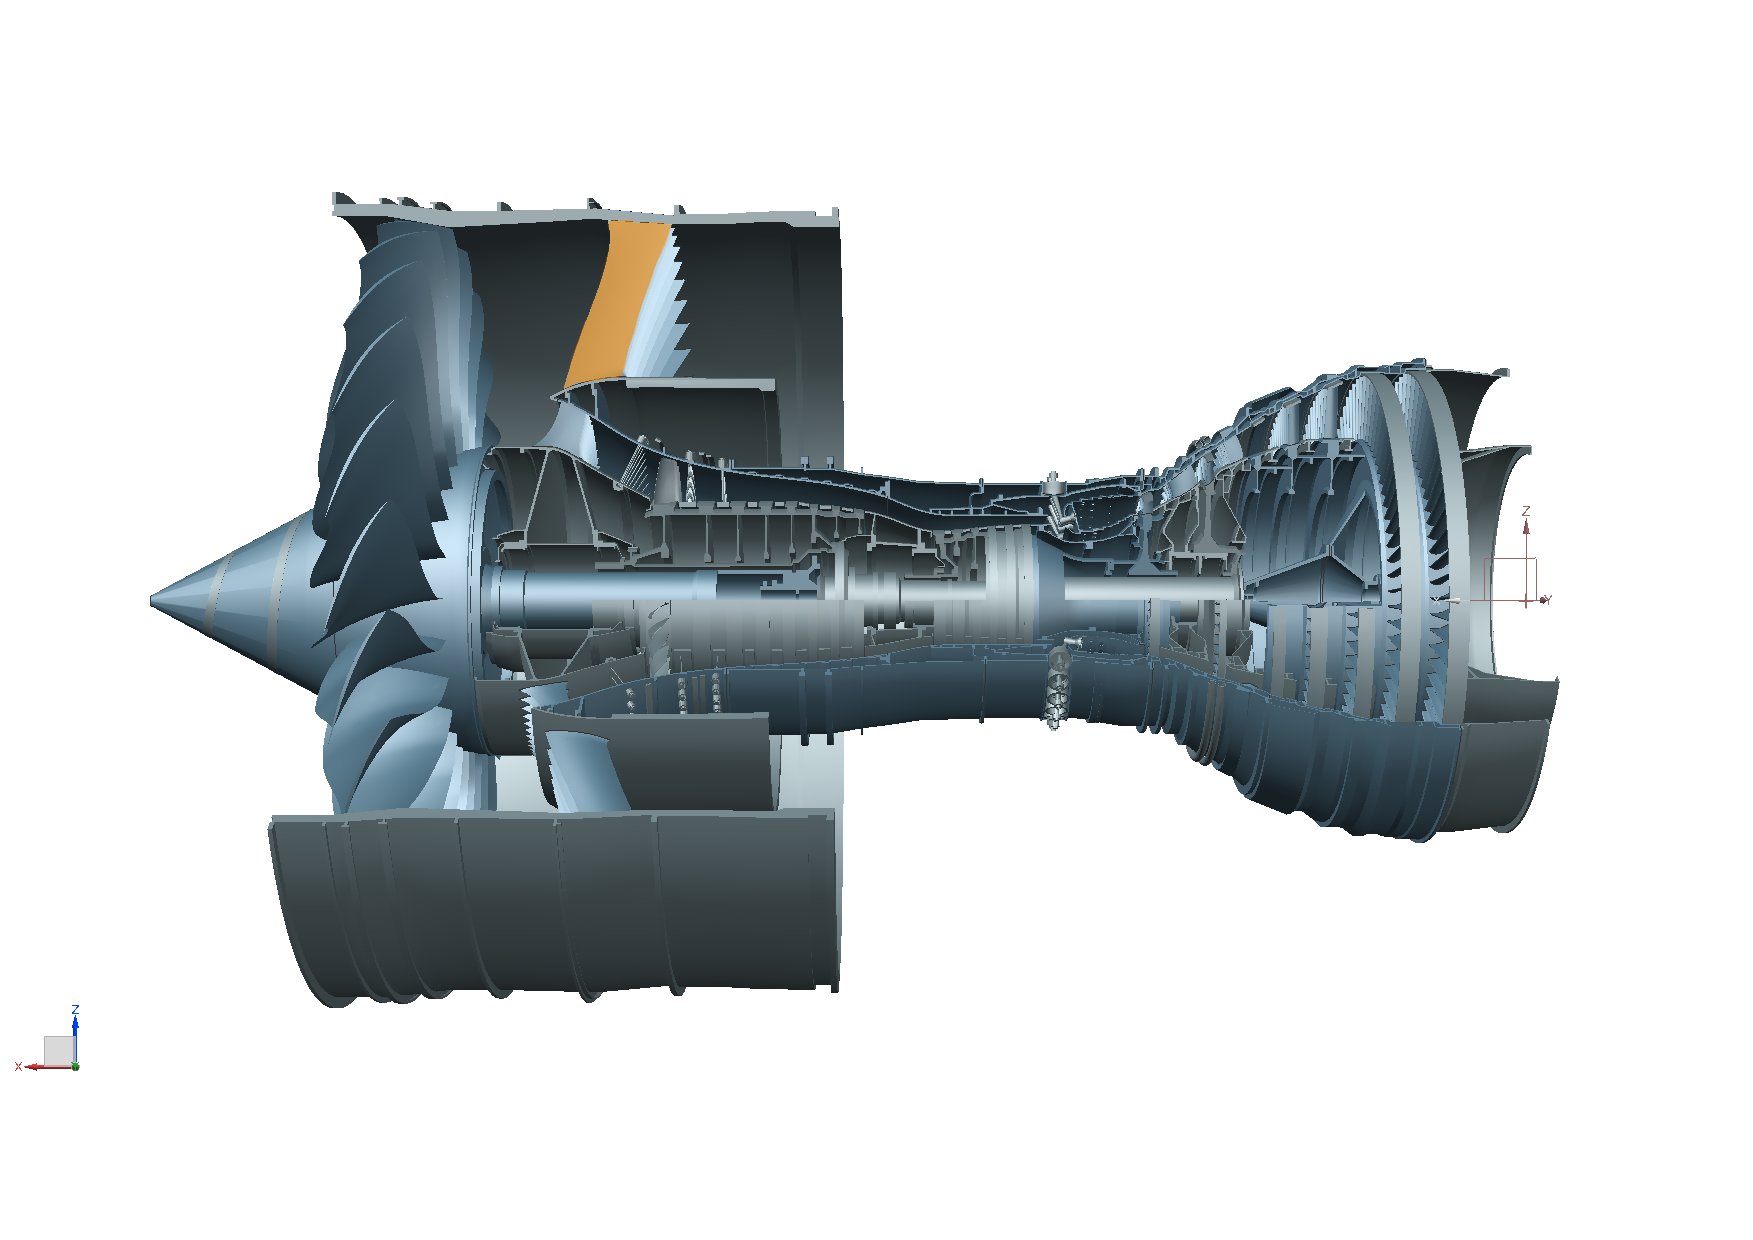
\includegraphics[width=.8\textwidth]{figures/trent9000_OGV.png}

        \caption{A Rolls Royce Trent 900 engine rendered in CAD\protect\footnotemark, with one GV highlighted in orange.
        }
        \label{fig:turbine}
    \end{center}
\end{figure}

\footnotetext{CAD model by Chris Shakal on grabcad.com}
%\Jakob{present an illustration of the simple sample vane, geometry and EF-M}

A \ac{GV} commonly consists of a vane structure, a predominantly aerodynamically defined structure, and two end attachments which fasten the vane to the engine core on the inside, and the outer fan case on the outside, as can be seen in Figure \ref{fig:turbine} and Figure \ref{fig:decompositionExample}.
Both parts provide interfaces the \ac{GV} assembly has to comply to.

%In the case company, the part is currently under redesign and development by a multidisciplinary team of more than ten engineers.
The development team is composed of both design and analysis engineers with experience in aerospace engineering ranging from five to thirty years.
These engineers partake in the development in defined percentage of their work-time, between 10\% and 70\%. 
\\

It is important to mention that the company is using and developing  \ac{KBE} techniques with a high degree of \ac{DA} for design space exploration.
This means that the engineers possess a benchmark system for comparison with the FGE. 
The benchmark system can be compared in make-up and extend to the parameterisation-based \ac{MDA} framework presented in \cite{Sandberg2017ADesign}.


\subsection{Study setup}
% action research framework
The research has been performed as a participatory action research study, where the researchers accompany the development process investigating into new opportunities for a fan frame \ac{GV} \citep{Yin2006}.
The researchers participated in regular team meetings together with the design team, and had the ability to observe the engineers during their work.
Notes from these meetings and observations are part of the data supporting the presented results.


Beyond the observation throughout the product development project, a set of studies has been conducted to investigate the perception of the presented method.
For the specific  purpose of validating the FGE method and tool, two consecutive workshops were organised together with the design team. 
% initial interviews???

% workshop 1 and decomposition
In a first workshop together with the \ac{GV} development team (eight participants), a functional decomposition of the part was performed and captured.
Hence, this workshop is referred to as the "decomposition workshop".
The actual workshop was predated with a one hour long test-workshop in one of the regular team meetings to evaluate the motivation of the practitioners and the requirements for the actual workshop.
The results of this "test-workshop" are included in the results of the decomposition workshop.
The decomposition was performed using large-scale print-outs of drawings a \ac{GV} which were annotated in a group exercise.
The annotated drawings were collected, digitised and used for the creation of function-geometry model in \ac{FGE} for the legacy design.
%After the decomposition activity, the practitioners were asked to fill out a questionnaire about their perception of the workshop.
%The workshop was concluded with an open feedback round.

%workshop 2
A second workshop (eight participants) covered the innovation stage of the \ac{FGE} approach. 
The workshop was held with the same development team, using the same product.%, although due to scheduling challenges the participant groups in workshop one and two were not exactly identical, but each engaged 80\% of members the development team.

% prototype tool
For the second, online\footnote{The workshop was performed online due to the social distancing regulations caused by the COVID-19 pandemic.}, workshop, a proof-of-concept tool of the \ac{FGE} approach was created.
The tool works server-based with a web interface (illustrated in Figure \ref{fig:omfgDSEinterface}), allowing users with different skill levels and operating systems to connect to the same database.
The tool incorporates a fully functional implementation of an \ac{EF-M} modeller with additional functionality to capture geometric information for each \ac{DS}.
As such, it is able to capture alternative design solutions and instantiate them into different concepts.
Furthermore, the tool include a geometrical modelling algorithm to automatically generate \ac{CAD} models of each concept, based on previous geometrical modularisation in Siemens NX.
The structure and mechanics of the tool are illustrated in \cite{Muller2021FunctionVariants}.

% data capture and analysis
After each workshop, the practitioners were asked for their experiences through questionnaires and open feedback.
The results of the first workshop were recorded through adhesive notes and remarks on the drawings, as well as protocol notes.
The results of the online workshop were captured through audio and video recording and through a change protocol in the database of the \ac{FGE} tool.

%The findings from the workshop were verified through semi-structured in-depth interviews with selected participants of the workshop. \Jakob{these are still outstanding - hopefully after summer!} 

%Since the product is currently being in development at the case company, it underlies certain \ac{IP} and export restrictions. 
\revision{For this publication, a generic design of a GV was created, which differs from the design used in the workshops.
However, the generic design has a sufficient degree of realism to enable dialogue, but with company specific features left out.}
%Therefore, a simplified model is used for presentation purposes in this publication in order to protect the case company's and their customers' \ac{IP}.
% 
%However, the simplified \ac{GV} model has been verified with the practitioners in order to be able to convey the main functions and solutions of a generic \ac{GV}.



%%%%%%%%%%%%%%%%%%%%%%%%%%%%%%%%%%%%%%%%%%%%%%%%%%%%%%%%%%%%%%%%%%%%%%%%%%%%%%%%%%%%
%%%%%%%%%%%%%%%%%%%%%%%%%%%%%%%%%%%%%%%%%%%%%%%%%%%%%%%%%%%%%%%%%%%%%%%%%%%%%%%%%%%%
%%%%%%%%%%%%%%%%%%%%%%%%%%%%%%%%%%%%%%%%%%%%%%%%%%%%%%%%%%%%%%%%%%%%%%%%%%%%%%%%%%%%
\section{Results}\label{sec:results}
\revision{This section presents the results of the application of FGE in the industrial context as well as the practitioners feedback and observations.}

%The next sections describe how the design space exploration of the GV has been conducted with the industrial practitioners with the support of FGE. 
%Also, it will describe the practitioners' feedback and reflections after the use of the method.
%The respective CAD models of the demo-geometry are shown in \ref{fig:}.

\begin{figure}[ht]
    \centering
    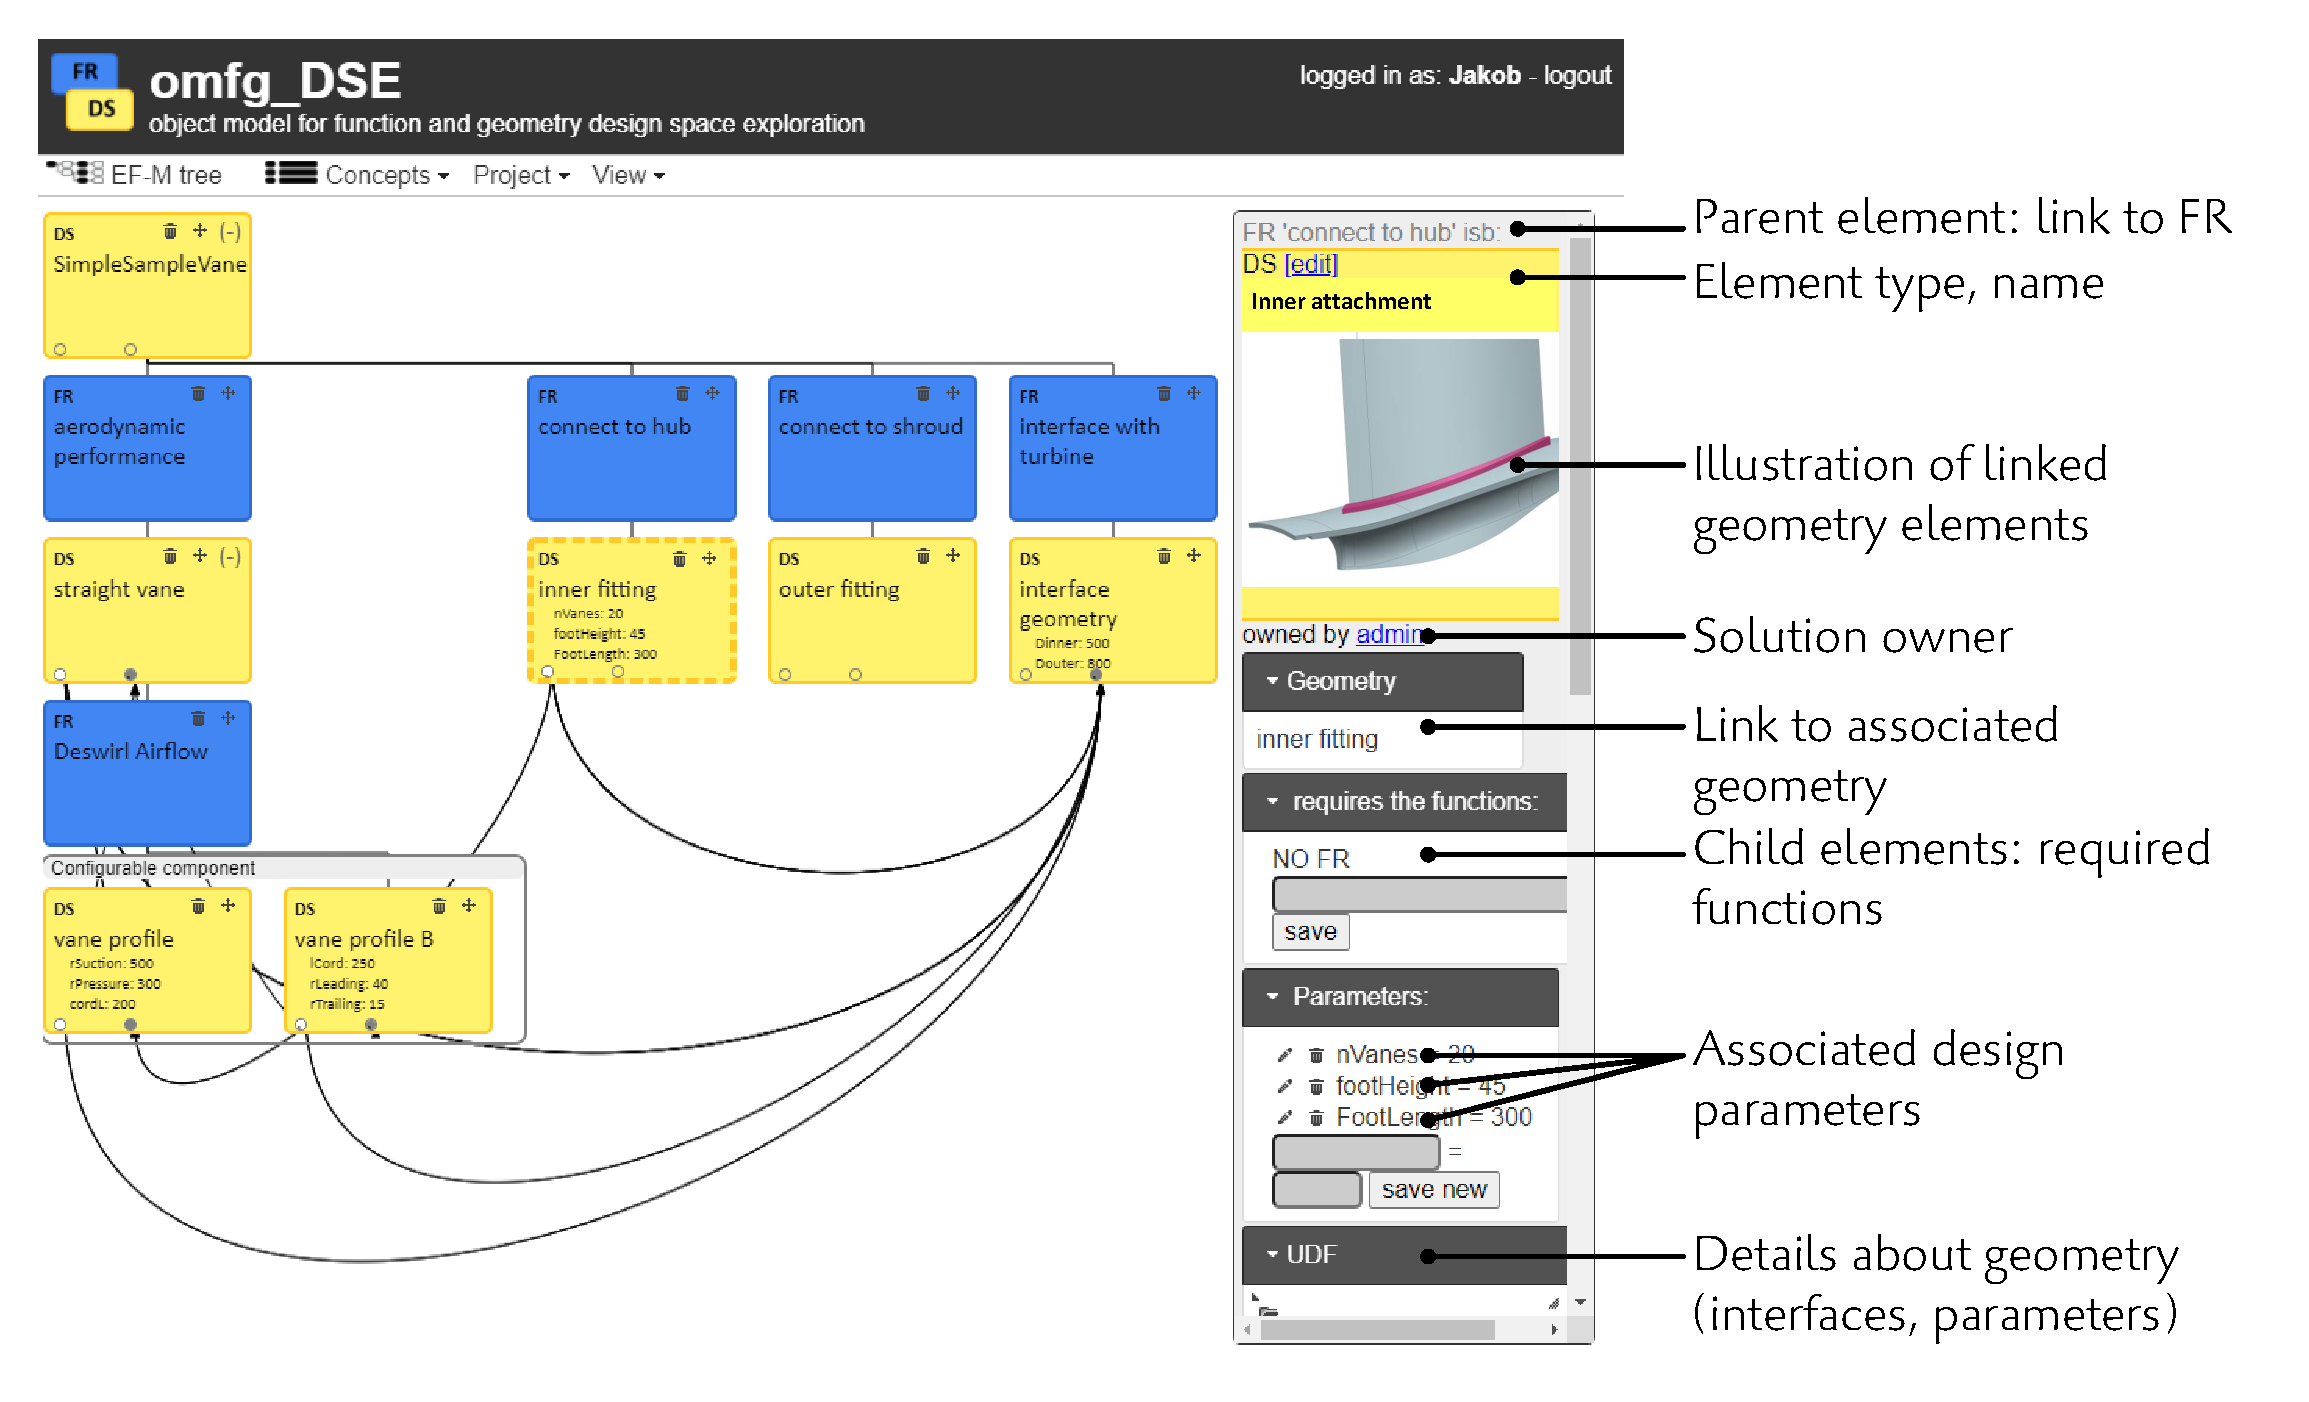
\includegraphics[width=\textwidth]{figures/pdf/interface.pdf}
    \caption{Web-based interface of the FGE tool "omfgDSE" (object model for function and geometry based design space exploration) , showing a simplified EF-M model of a GV.
    The right-hand pane illustrates the design rationale of the selected DS, such as associated function, geometry and parameters.}
    \label{fig:omfgDSEinterface}
\end{figure}

%%%%%%%%%%%%%%%%%%%%%%%%%%%%%%%%%%%%%%%%%%%%%%%%%%%%%%%%%%%%%
\subsection{Design space exploration using FGE}
The \ac{DSE} approach is separated into three phases \textit{decomposition}, \textit{innovation} and \textit{embodiment}, following \cite{Muller2019Aiedam}.
The presented workshop focuses on the interactions with practitioners in the phases decomposition and innovation.

% Decomposition
%\subsubsection{First workshop - Decomposition}

In the first workshop \textit{(decomposition)}, the legacy design of the \ac{GV} was captured in an \ac{EF-M} model based on the available geometry.
The model contains three main functions, and 18 different design solutions on the concrete (lowest) level.
Since the model was created through decomposition, all \ac{DS} are directly linked to one or several geometry elements.
A modularised CAD model was created based on the original geometry, modularised according to the decomposition.
% introduce here the new figure

% \begin{figure}[ht]
%     \centering
%     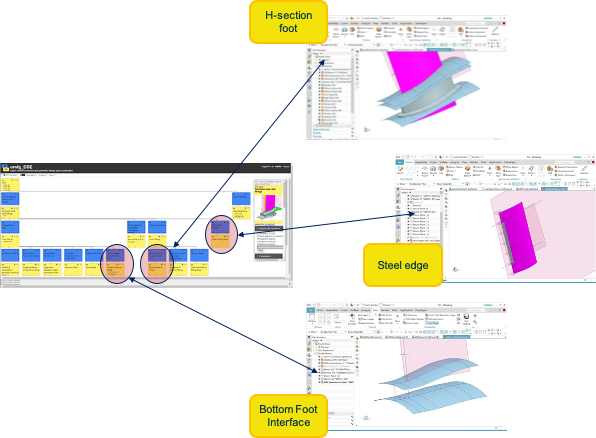
\includegraphics[width=\textwidth]{Picture 2.png}
%     \caption{Connection between the modularized CAD model of the legacy design, directly linked to the DSs in the EF-M model.}
%     \label{modularizedCAD}
% \end{figure}

\begin{figure}[ht]
    \centering
    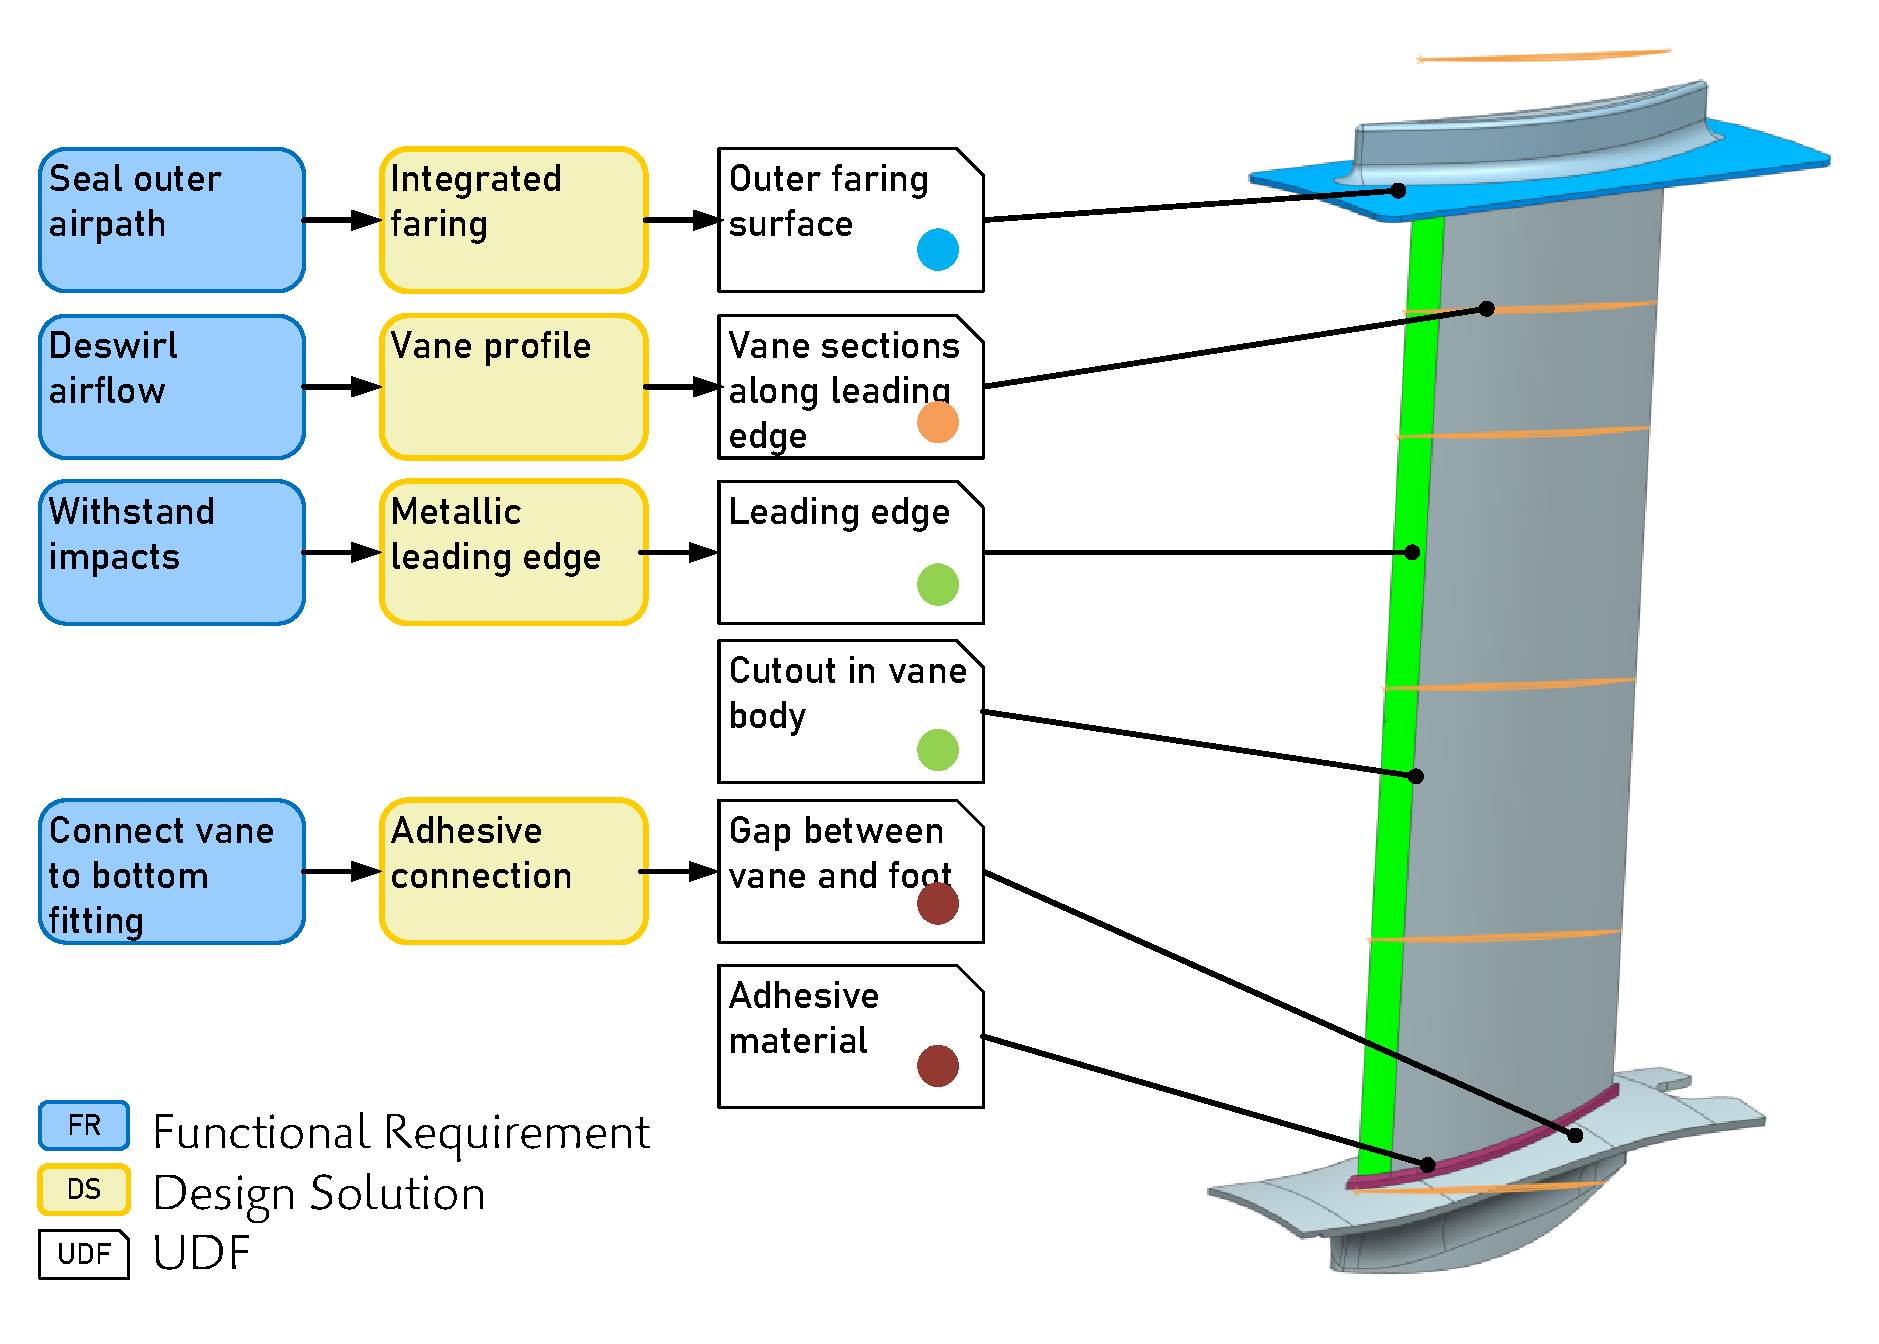
\includegraphics[width=\textwidth]{figures/pdf/ogvDecomp.pdf}
    \caption{Example of function and design solutions of a GV, connected to geometry elements as UDF.
    The different geometry elements are colour coded to show the extend of the UDF.}
    \label{fig:decompositionExample}
\end{figure}

Figure \ref{fig:decompositionExample} exemplary shows this modularisation and connection for four individual \acp{DS} and the related \acp{UDF}.
For example, the leading edge of the decomposed \ac{GV} is covered by a metallic edge.
This \revision{metallic}  edge, as a geometrical element, has been associated with the function "Withstand impacts" through the solution "Metallic  edge".
The respective geometry, of both the edge insert and the cutout in the vane to place it in, are captured as two \acp{UDF} which are then associated with the \ac{DS}.


%Other examples of geometry elements connected to DSs are "H-section foot" and "Bottom Foot Interface". 
This decomposition served as input for the following workshop, focused on innovation. 
\\


% introduce here a connecting sentence witht he next 
% new solutions
%\subsubsection{Second workshop - Innovation}

In the second workshop \textit{(innovation)} the prototype tool was used to capture novel design solutions.
As a result, the product model was extended by five new sub-functions with their respective solutions and 10 new alternative \ac{DS}.
As an example for new FR, sub-functions related to acoustic performance were added to the model. 
%In the workshop, the practitioners found ten novel alternative  design solutions over the legacy design.
The nature of the \ac{DS} ranged from material alternatives over different interface approaches to variations in shape and dimensions of the existing solutions.
The entire EF-M tree, with all new FR and DS highlighted with red borders, is shown in Figure \ref{fig:fullEFM}.
Based on the new alternative DS, 52 different concepts could be instantiated.


% new solutions example
The majority of the novel solutions shows a conceptual difference from the legacy design.
As an example, the \ac{FR} "Join vane to attachment" is in the legacy design solved by the \ac{DS} "Adhesive connection", meaning that the vane is glued to the attachment using resin.
This DS, and the respective UDF, are illustrated in Figure \ref{fig:decompositionExample}.
The two alternative \ac{DS}, as results from the workshop, were "Bolted joint" and "Fully integrated solution".
The respective DS are shown in Figure \ref{fig:efmAltFoot}, whereas the geometry related to these DS is shown in the context of the GV in Figure \ref{fig:altGV}.

%subsubsection{Embodiment}
% maybe we should not bring this:
The \textit{embodiment} phase of the \ac{FGE} approach has not been performed in its entirety, since the \ac{DA} section of the proof-of-concept tool has not sufficiently matured to handle the complex geometries of the solutions devised in the innovation workshop. For a verification of the proof-of-concept tool on another turbine structure, see \citep{Muller2021FunctionVariants}.

% alternative:
% Based on the different alternative solutions and functions captured in the innovation workshop, 52 different concepts were instantiated.
% The respective solutions were embodied and combined.

Figure \ref{fig:altGV} shows an exemplary embodiment of three concepts with alternative DS for the FR "Join vane to \revision{attachment}" shown in Figure \ref{fig:efmAltFoot}.
While otherwise using the same configuration, each of the geometries is adapted to accommodate the respective geometric changes in the concept.
The instantiation and assembly algorithms embedded in the FGE model allow for automated generation of the CAD models of all feasible concepts.  

\begin{figure}[ht]
    \centering
    
        \begin{subfigure}[b]{0.6\textwidth}
            \centering
            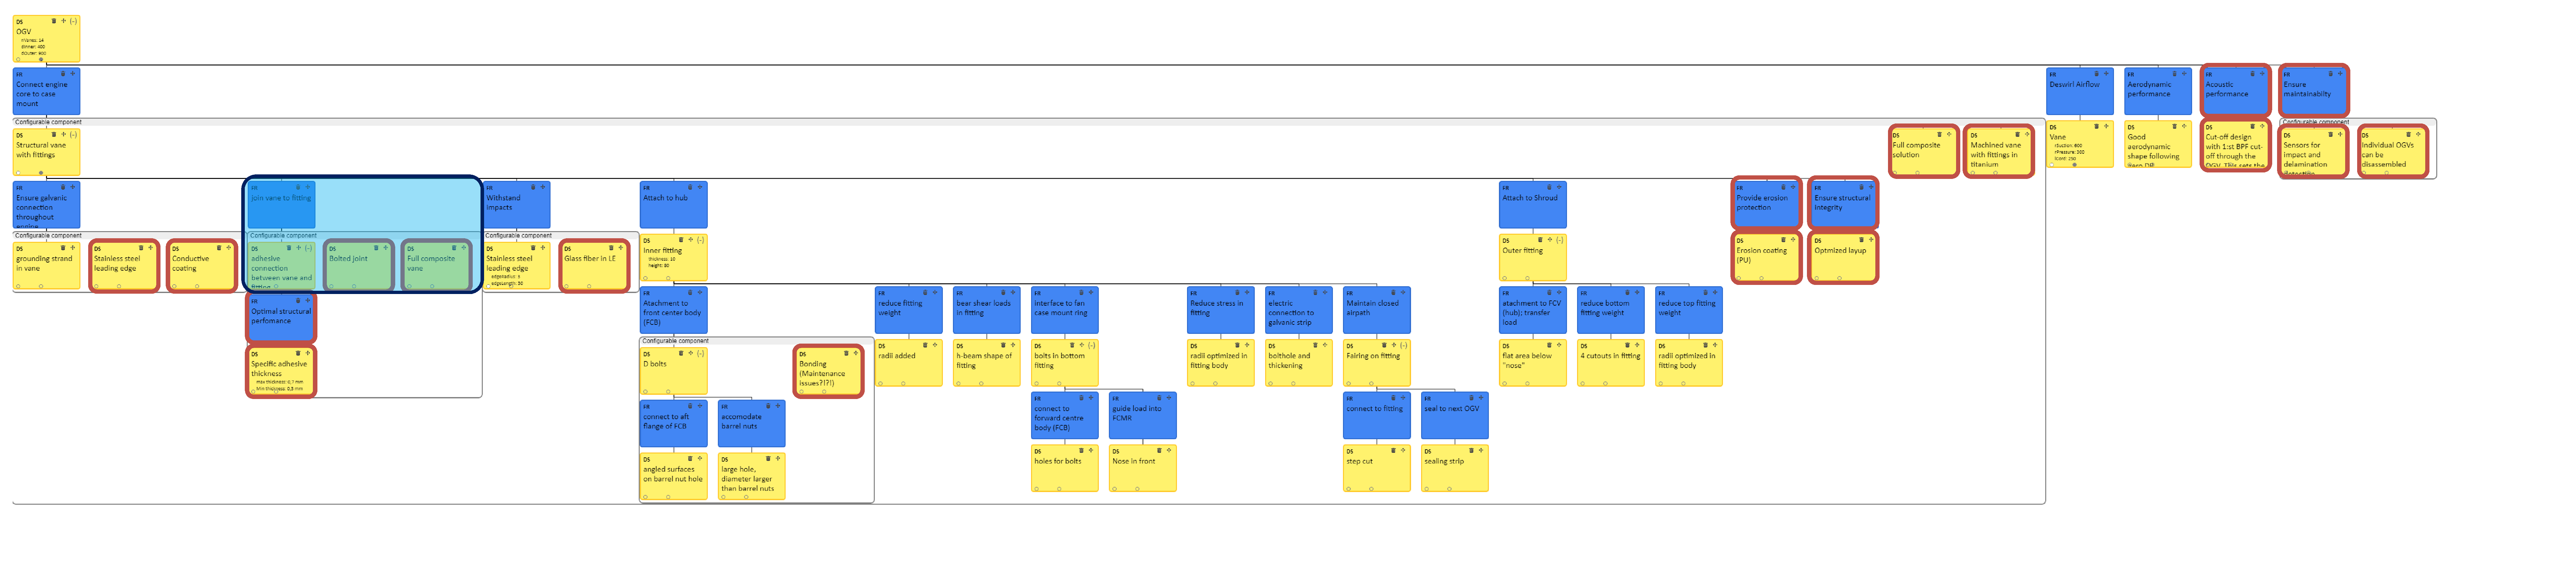
\includegraphics[width=\textwidth]{figures/pdf/fullEFM.pdf}
            \caption{}
            \label{fig:fullEFM}
        \end{subfigure}
        \hfill
        \begin{subfigure}[b]{0.35\textwidth}
            \centering
            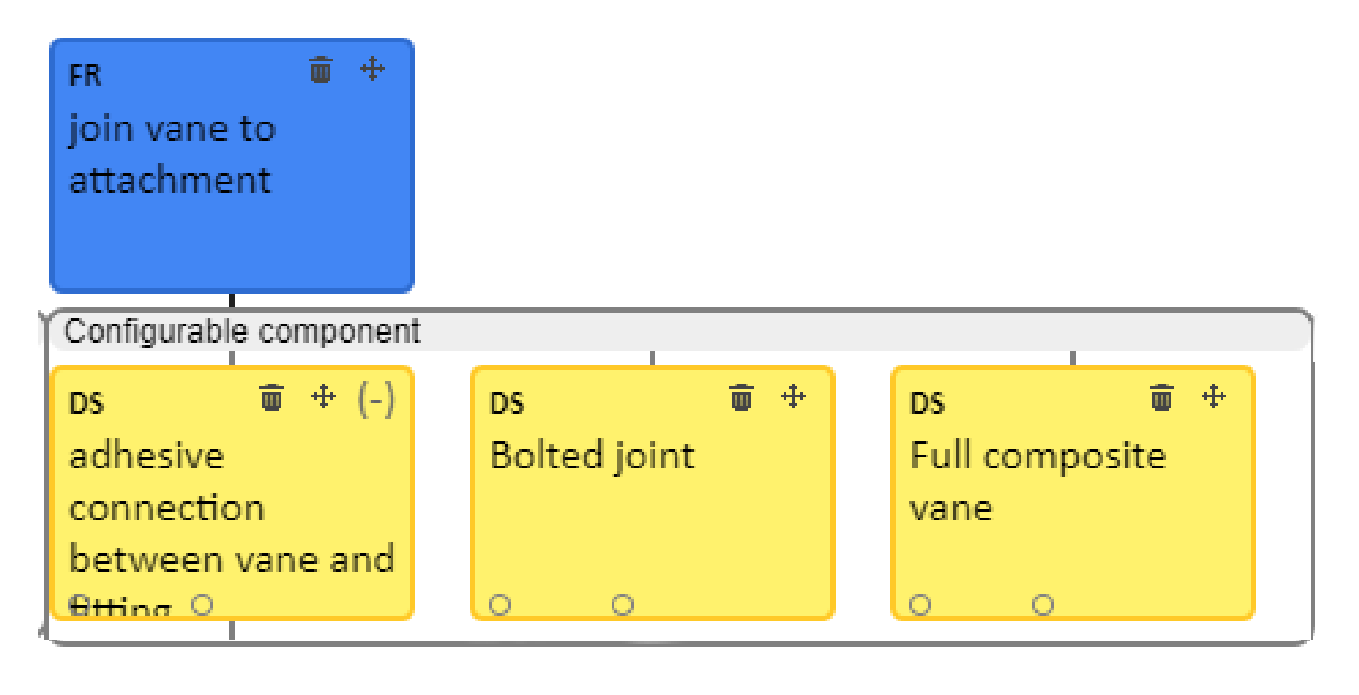
\includegraphics[width=\textwidth]{figures/pdf/efmDetail.pdf}
            \caption{}
            \label{fig:efmAltFoot}
        \end{subfigure}
        
    \caption{EF-M model after the innovation workshop.
    (a) Full EF-M tree, with all new DS and FR highlighted with a red border.
     Readability has been dismissed on purpose to protect company IP.
    (b) Detail: alternative solutions for DS "Join vane to attachment", highlighted in blue in (a).}
    \label{fig:efmResults}
\end{figure}


\begin{figure}[th!]
    \begin{center}
    \centering
        \begin{subfigure}[b]{0.3\textwidth}
            \centering
            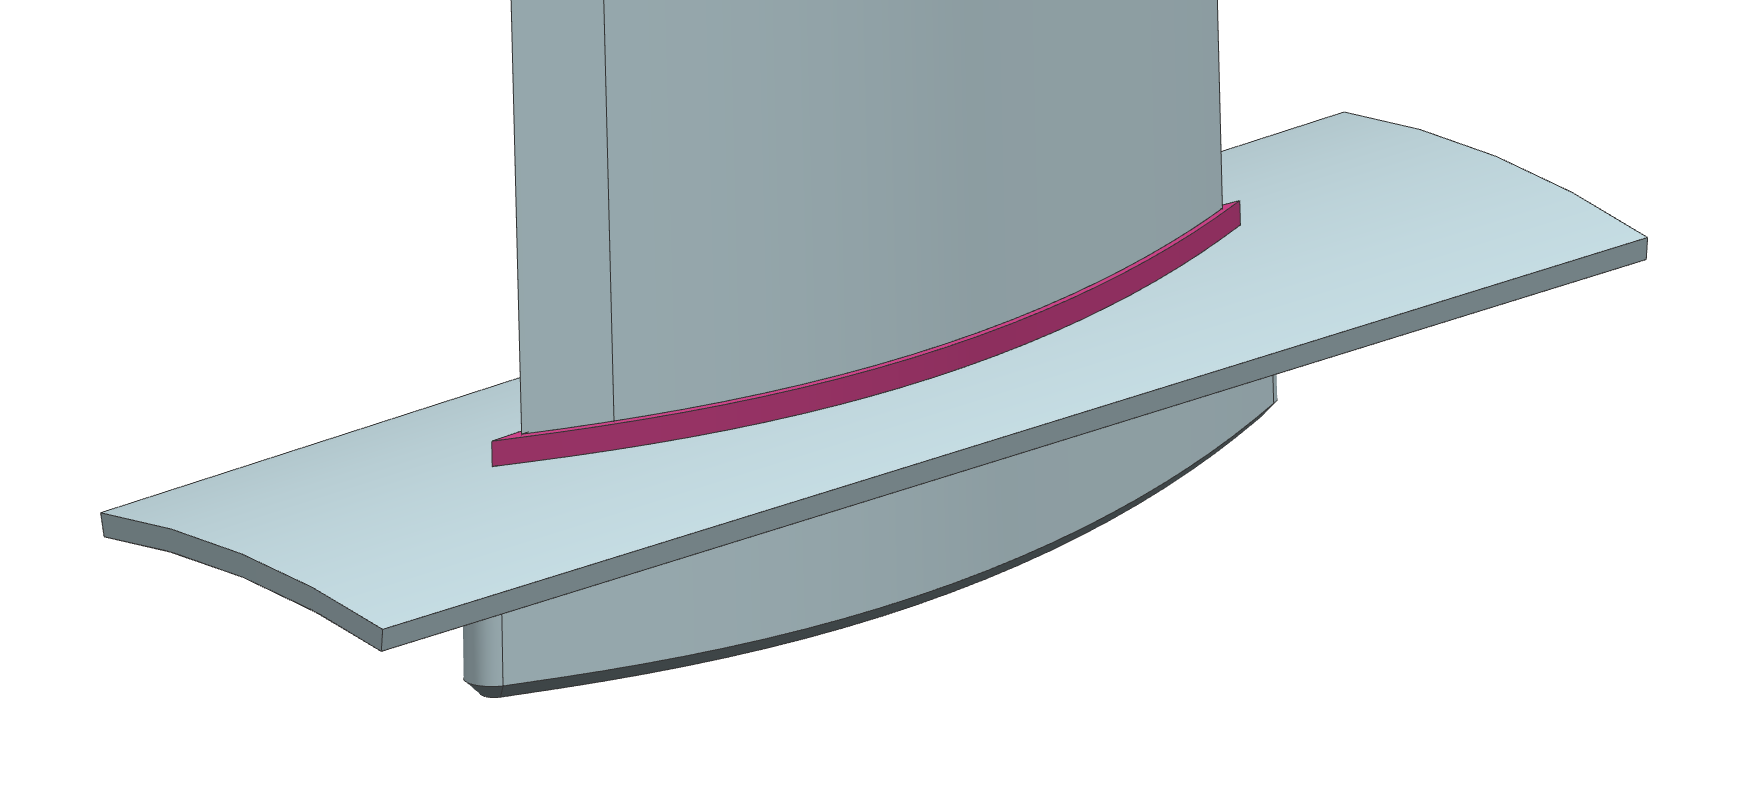
\includegraphics[width=\textwidth]{figures/van2.png}
            \caption{}
            \label{fig:footGlued}
        \end{subfigure}
        \hfill
        \begin{subfigure}[b]{0.3\textwidth}
            \centering
            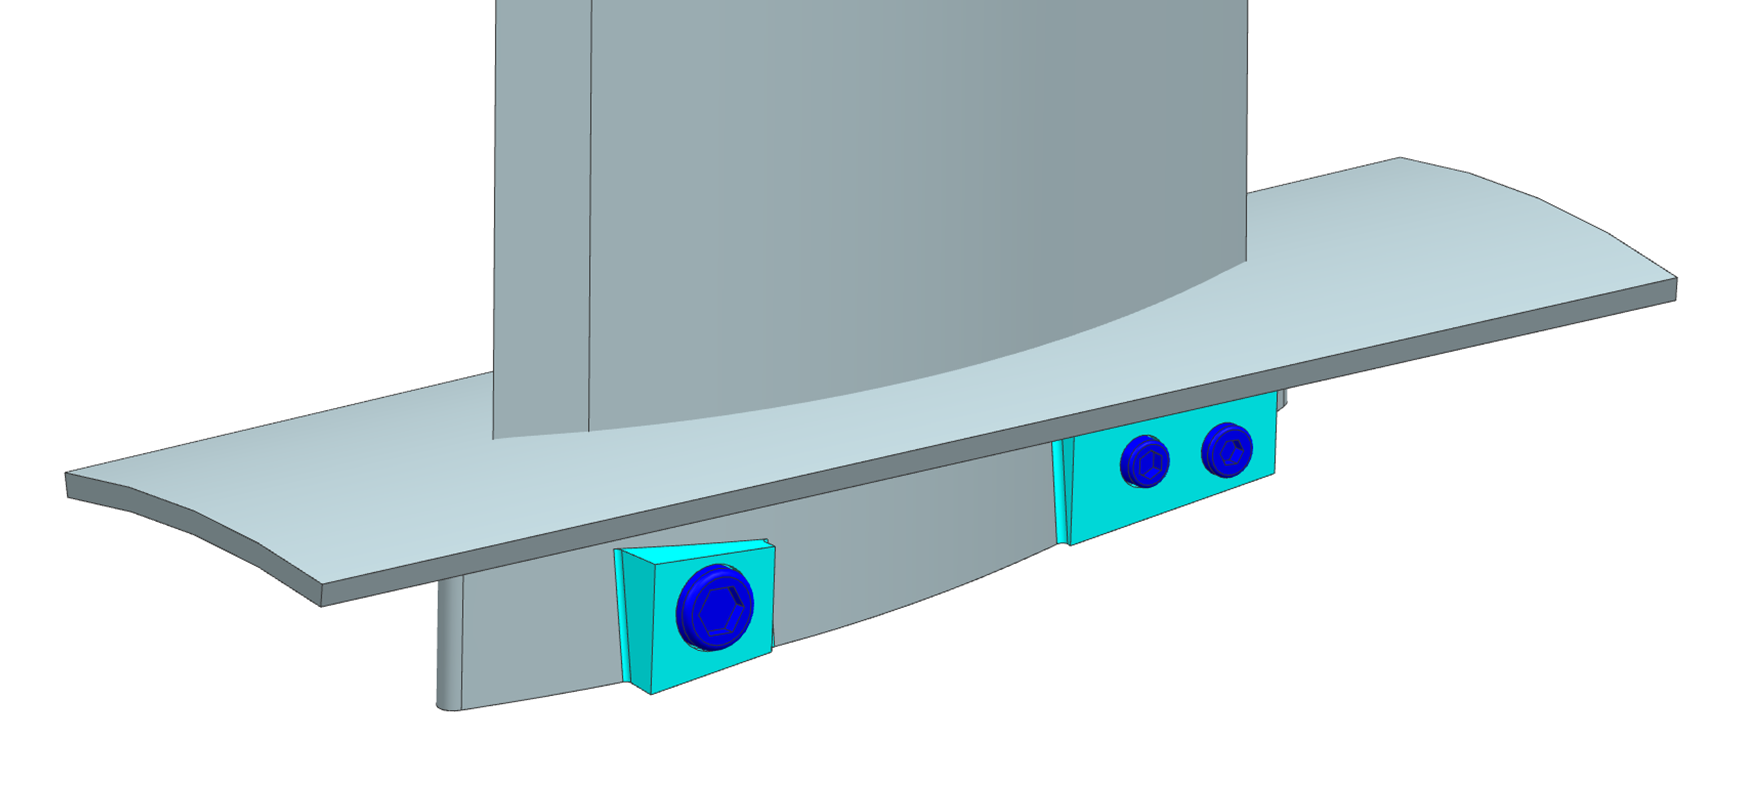
\includegraphics[width=\textwidth]{figures/vane1.png}
            \caption{}
            \label{fig:footBolted}
        \end{subfigure}
        \hfill
        \begin{subfigure}[b]{0.3\textwidth}
            \centering
            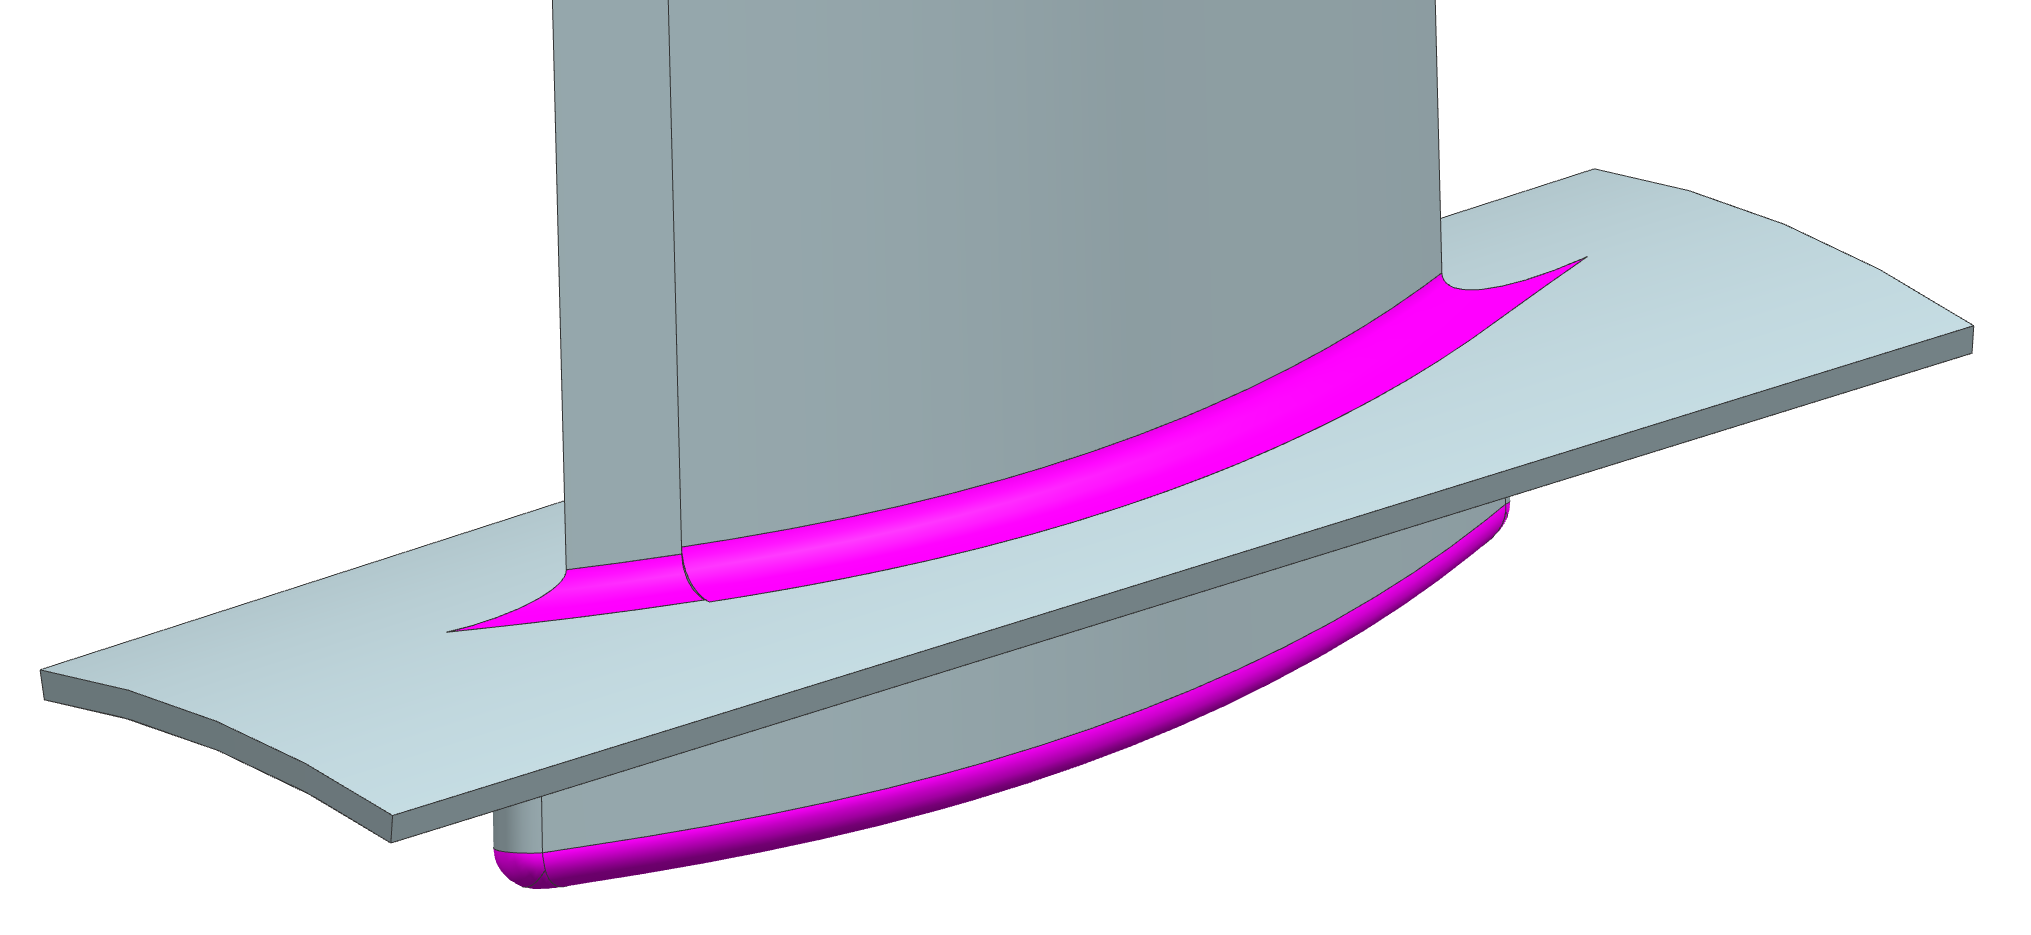
\includegraphics[width=\textwidth]{figures/vane3.png}
            \caption{}
            \label{fig:footOnepice}
        \end{subfigure}
        \caption{Embodiment of three concepts, differentiating in the solutions for the FR "Join vane to \revision{attachment"}, from left: (a) "Adhesive connection", (b) "Bolted joint" and (c) "Fully integrated solution".
        Respective alternative geometric elements relating to the respective UDF are highlighted in colour.}
        
        % \caption{Embodiment of three concepts, differentiating in the solutions for the FR "Join vane to fitting", from left: (a) "Adhesive connection", (b) "Bolted joint" and (c) "Fully integrated solution".
        % Respective alternative geometric elements relating to the respective UDF are highlighted in colour.}
        \label{fig:altGV}
    \end{center}
\end{figure}


The following section reports on the practitioners' feedback and reflections after the application of the method on their industrial use case. 

% Each of the solutions was modelled as a \ac{UDF} in Siemens NX, and the resulting UDF was coupled to the EF-M model through the \ac{OMFG}.
% %The resulting \textit{UDF} and \textit{interface} objects in the \ac{OMFG}, as well as the geometry, are illustrated in Figure \ref{fig:altSolutionOmfg}.

% % instantiated 
 % geometry
% The technical feasibility of automated geometry generation was assessed based on experiences with the \ac{FGE} modelling approach in a previous study with a similar turbofan engine part, see \cite{Muller2020a}.
% This qualitative assessment of the new concepts showed that approximately $35$ of the 52 theoretically possible concepts could be realised as CAD models, using the modular \ac{DA} approach of \ac{FGE}.
% \Jakob{
% In the workshop, 10 relevant new DS were introduced (compared to legacy design)

% 2 new functions were introduced

% total of 52 new concepts

% how many of these geometrifiable?

% }

%%%%%%%%%%%%%%%%%%%%%%%%%%%%%%%%%%%%%%%%%%%%%%%%%%%%%%%%%%%%%
\subsection{Reflections form industrial practitioners regarding the application of the method} \label{sec:feedback}

The practitioners have stated that the workshops---as design activities in addition to their regular design activities---contribute to the development project.
%albeit it was maybe too late in the development process.
Furthermore, all workshop participants would like to repeat the workshop concept, both in the same, but even more so in other projects.
The following sections will go through the main mechanisms that have been highlighted by the industrial practitioners, in particular the ability of the approach to:

\begin{enumerate}
	%\item Provide a clear and explicit illustration of the design rationale of the product. 
	\item Represent and capture design rationale and the design space
	\item Capture, integrate and model novel solutions
	%\item Provide a clear connection between the abstract functional and the concrete geometrical domain, which has the potential to foster innovation.
	\item Provide support for the embodiment of novel concepts that would otherwise remain unexplored
\end{enumerate}

\subsubsection{Capture and representation of design rationale and design space}

\begin{center}
    “I learned a lot of things about the GV just by reading the graph” 
\end{center}
\begin{flushright}
    -aerodynamics analysis engineer
\end{flushright}


This quote illustrates a common problem during the design of aerospace products.
As components are designed and conceptualised over long times, and by heterogenuous teams, it is difficult to retain the \acf{DR} of a product (that is, why a product has been designed in this form) \citep{Bracewell2009}. 
This \ac{DR} is especially hard to read in highly integrated and complex products such as aerospace engine components, where a single geometrical artefact may fulfil multiple functions in different domains \cite{Raja2019}.
For practitioners, the FGE approach supports the ability to visualise the rationale in both the geometrical domain, visualising "what is", and the functional domain, "why it is".

In terms of the use of \ac{FGE}, it appears to be a major benefit of FGE for the practitioners that they improved their knowledge about the product and participated in a forum that permitted exchange about the product's functions and solutions.
The questionnaire accompanying the workshop revealed that no team member had full confidence about the \ac{GV}, but most rated their understanding of the GV higher after the workshop than before.
The workshop also fostered the awareness of \textit{meta-product-knowledge}, since many engineers were not even aware \textit{who} knew the rationale behind a specific element.
Only through discussions and participation of engineers of multiple disciplines could the entire DR be captured in the EF-M model.


An example for how \ac{FGE} enables access to \ac{DR} is the interface of the tool used in the study, which collects all information of a solution in a single place.
Figure \ref{fig:omfgDSEinterface} shows on the right hand side how the geometry, parameterisation and other information about a solution is collected in a single window pane.
The top of the pane shows which function is solved, and the highlighting of the solution shows its position in the product architecture.

Furthermore, the approach can illustrate the geometrical interfaces between solutions through \ac{iw} connectors in the \ac{EF-M} model.
This are seen as black arcs in the interface of Figure \ref{fig:omfgDSEinterface}, left hand side.

This approach of information representation was referred to as "comprehensive" by the workshop participants.

% tree / alt solutions in EF-M
Beyond the information about individual solutions, the \ac{FGE} interface provides an overview over the possible alternatives through \ac{EF-M}.
This was perceived to be an efficient way to represent the design space, providing "good possibilities to look at different solutions".
However, it was also noted by one participant in the workshop that the function models can quickly grow to be too complex.
The function model created in this study (see Figure \ref{fig:fullEFM}) was considered "almost too large".

%Proofing this, most practitioners stated a higher knowledge of the product after the workshop than before.



%please comment the figure.
%redid the figure to hide the IP information and show iw connectors
% have to enlarge it though for readbility -.- but that takes too much time now
%also think i embedded it in the text ok?

%%%%%%%%%%%%%%%%%%%%%%%%%%%%%%%%%%%%%%%%%%%%%%%%%%
%%%%%%%%%%%%%%%%%%%%%%%%%%%%%%%%%%%%%%%%%%%%%%%%%%
\subsubsection{Ability to capture, integrate and model novel solutions. }

\begin{center}
    “Parametric solutions exist but limited to parameters that we easily can change, dimensions, angles or thicknesses for example.  When it comes to exploring different design solutions in early phases we foresee larger challenges.” 
\end{center}
\begin{flushright}
    -- development team leader
\end{flushright}

% \begin{center}
%     “Right now our system for DSE is limited to changing parameters (dimensions, angles…) and does not iterate over different Design solutions” 
% \end{center}
% \begin{flushright}
%     -- analysis/meshing specialist
% \end{flushright}

This quotes stands exemplary for the practitioners' reflections over the in-house \ac{KBE} system for DSE adopted by the company, which is built around state of the art KBE approaches.
However, the practitioners are well aware about the limitations of highly automated CAD approaches in representing conceptually different design solutions.
While the exploration of dimensional variety is possible and appreciated by the practitioners, the need to realise topologically and geometrically different options has been stated explicitely.
This matches with observations from literature, where it is stated that "a parametric model offers little flexibility" \cite{Li2020UsingIntegration}.

According to the practitioners, FGE has the potential to deliver this through the modularisation of the geometry, and the connection to the \ac{DR} of the product.

% more solutions
It was perceived by the participants of the workshop that the use of the \ac{FGE} approach supports the introduction of new solutions ($4$ on a scale of $1$ "no support for new solutions" to $5$ "totally supports").
% novel solutions
It was furthermore stated that a part of the identified \ac{DS} would probably not have been found -- or considered -- in a regular modelling approach, with a majority ($71\%$) stating "maybe some, but not all".
The other participants stated either "none of them" or "most of them" would have been identified without \ac{FGE}.

% more functions 
Beyond only exploring new solutions for existing functions, \ac{FGE} also enables the capture of newly identified functions or sub-functions.
The workshop results showed that through five new functions being identified during the innovation workshop.
Practitioners feedback further supported this, although the ability to integrate new solutions is perceived to be more important than that of new functions.

To summarise this, the practitioners perceive FGE as a viable method to capture novel solutions and functions.
Having a formal, and even computer  supported, modelling approach at hand when generating conceptual alternatives directly in creative design meetings was found very applicable. 




%%%%%%%%%%%%%%%%%%%%%%%%%%%%%%%%%%%%%%%%%%%%%%%%%%
%%%%%%%%%%%%%%%%%%%%%%%%%%%%%%%%%%%%%%%%%%%%%%%%%%

\subsubsection{Support for the embodiment of novel concepts}


% \begin{center}
%     “What we are looking for is how to get an efficient concept generation phase before we go into our parametric system [\textit{author's note: the in-house systems for DSE}]  –- so that we get an overview over potential concepts” 
% \end{center}
% \begin{flushright}
%     -- development team leader
% \end{flushright}


\begin{center}
    “There are still gaps within early concept phase – this is one possibility to generate, and evaluate, lots of concepts, get trend curves and so on.” 
\end{center}
\begin{flushright}
    -- design engineer
\end{flushright}

% Especially in aerospace components, due to strict constraints on weight and high requirements on performance, the products turn out to be highly integrated \citep{Raja2019}.
% As a result, only few team members have an overview over the \ac{DR} of the product. 
% This has also been observed in the workshops.
% Only one team member was relatively confident in their knowledge about the part, whereas the others had only segmented knowledge and judged their knowledge with an average of 2.7 out of five.

% FGE good
As has been stated in the section above, there is a substantial need for a \ac{DSE} modelling approach to capture geometrically and topologically different \ac{DS}.
The practitioners agree that \ac{FGE} is an approach which can support such exploration.

% CAD needed
However, the sole representation of alternative concepts in function models would be insufficient.
To enable the necessary analyses, geometry models in the form of CAD are required.

% required CAD qualities
The practitioners stated that the CAD models needed for effective \ac{DSE} need to be of sufficient quality to be meshed automatically.
This requires certain quality criteria such as surface continuity.
Furthermore would the CAD models require automated "tagging" of relevant geometry elements for analyses, for example where forces attack or constraints apply.


% possible with FGE
After a demonstration of the assembly algorithm of FGE and the geometry modularisation, the practitioners agreed that such an approach can deliver the required models.
Therefore, the ability to generate \textit{topologically different} variant concepts was seen as a benefit of the presented method.

%identified areas for improvement through decomposition as well as identified "do not touch"
% Almost all participants stated that through the decomposition workshop, "do not touch" areas as well as areas for improvement on the product could be identified.
% This provides a clearer representation of the design space for the engineers: 
% through the mapping of geometry to function, the "do not touch" areas become tangible in \textit{why} they shouldn't be altered, and furthermore what impact this has on the rest of the product architecture, with a participant representatively stating it was interesting to see "how it is connected"
% This is a major strength of the direct coupling of the function to the geometry model:
% Other modelling approaches do not represent how a requirement or constraint does impact the geometry.
% The motivation \textit{why} an area cannot be subject to altering is stored in the \textit{rationale} -- through the connection a geometrical element it becomes tangible,


% However, the need for discussion of these findings in follow-up meetings was also highlighted by most of the participants.
% This result is corroborated by the results of the questionnaire from the innovation workshop.


% \begin{figure}[ht]
%     \centering
%     \includegraphics[width=\textwidth]{figures/resultsInnov.png}
%     \caption{Selected answers from the questionnaire after the innovation workshop. Each $x$ represents one answer. If less than eight answers per question are shown, some participants did not answer.}
%     \label{fig:resultsInnov}
% \end{figure}


\begin{center}
    “generation of CAD models based on different configurations is a key functionality” 
\end{center}
\begin{flushright}
    -- development team leader
\end{flushright}




% On this regard, the \ac{FGE} framework has been evaluated as beneficial, especially if connected and integrated with the in-house systems for DSE, which supports an automated \ac{MDA} approach.
% The reason for this is that the analysis phases needs to rely on reliable meshing techniques, which are already supported by the in-house system for DSE.
% In this context, FGE is seen as a method to be used \textit{before} the in-house parameterisation and analysis tool.
% The integration with other systems to be used for detailed analysis is considered as an important aspect.
% However, the main benefit of FGE is on the ability t\textit{o generate and integrate more radical design concepts in the early phases}, from which a preliminary design analysis (even only based on expert opininon) can be conducted upon. 


%%%%%%%%%%%%%%%%%%%%%%%%%%%%%%%%%%%%%%%%%%%%%%%%%%
%%%%%%%%%%%%%%%%%%%%%%%%%%%%%%%%%%%%%%%%%%%%%%%%%%
\subsubsection{Implementation challenges }

Despite the interest on the approach, the practitioners pointed out certain implementation challenges.


As a feedback of the modelling process using \ac{EF-M} to capture and represent alternative solutions, a practitioner mentioned that the re-use of existing solution's geometry for another function is hardly possible to model using EF-M.
%If, for example, the \ac{FR} "Electric grounding of vane" uses the galvanic properties of the metallic leading-edge, this relation can hardly be represented in \ac{EF-M}.
Although there exist horizontal relations in EF-M modelling, they increase the modelling complexity and reduce readability.
%A workaround for this is to phrase the respective \ac{DS} "Use grounding vane" and model an \ac{iw} connection between them.
%However, the second \ac{DS} would always have to act as a 'slave' in respect to the first \ac{DS} from which it "borrows" product properties. 
Therefore, such complex relationship modelling has not been implemented yet in the prototype tool, and does not contribute to alleviate the challenges of complexity in function modelling stated by \cite{Muller2020, Tomiyama2013}.

The ratio of complexity between the functional domain and geometrical domain was point for critique.
It was stated that a large function model (such as the one in the workshop became through the innovation) reduces the overview over the model.
It was suggested to use less FR/DR elements and more, but potentially more complex, geometric modules.
However, the experience with function modelling and/or web-based applications may play a role in how difficult the tool use was perceived.

% redo for: need to couple FGE and EWB
While FGE supports the exploration of technically, functionally and topologically different solutions, the in-house KBE solution is optimised for parametric variation.
Being used to the already existing MDA method at the company, the practitioners rather viewed an implementation of FGE as a complement, preferably integrated with the existing system. 
% The attractive means of FGE, to explore the design space more flexibly, would be attractive to combine with highly automated and generative capabiliites already existing for variations of conceps. 
%Furthermore is the in-house KBE solution already set up with an automated \ac{MDA} tool-chain, which enables automated behaviour analysis.
% The practitioners have stated that a combination of both systems, with the in-house solution building onto the output of \ac{FGE}, would be the desired option for efficient \ac{DSE}.
% meshing
% While the automated generation of CAD models was very much welcomed, it was enhanced that this is only beneficial for the product development process if the models are of sufficient quality for downstream processes.
% Several participants stated the need for continuous model surfaces to be able to apply automated meshing routines.
% Furthermore was the need for markup in terms of analysis-relevant geometry elements (such as loaded or fixed surfaces) highlighted.





% I have commented out the whole section 3.2. just for makign easy the new editing 

%%%%%%%%%%%%%%%%%%%%%%%%%%%%%%%%%%%%%%%%%%
\section{Discussion} \label{sec:discussion}

The \ac{FGE} approach aims to support \ac{DSE} in the conceptual product development phases through a three-phase approach, namely decomposition, innovation and embodiment.
\revision{The approach relies on the \ac{OMFG}, which provides a connection between the previously divided modelling domains of \textit{function} and \textit{geometry}.
As a result, novel solutions can be integrated into an existing legacy design, and be embodied based on information stored in the function model.
This information, the DR of the product, is the driving force behind the implemented DA approach.
The coupling of the function and geometric modelling domain, and the resulting opportunities for DSE, distinguish the approach from other \ac{DA} approaches and CAD model parameterisation.}
The approach has been evaluated in a case study with a product development team of an aerospace manufacturer.

% validation of the gap
The practitioners gave an overall positive feedback about the approach, stating that \ac{FGE} -- or a similar approach -- can provide what is needed to improve current product development practice.
The need was stated to be about \textit{capturing} and \textit{presenting} alternative solutions in a systematic way, as well as an \textit{automated generation of CAD models} ready for analysis.
%These needs match with the aim of the \ac{FGE} approach, and are also stated in \ac{DSE} literature such as \cite{Kang2011}, who name ...
The use of a non-geometrical modelling approach representing teleological product knowledge, "how it all connects", has been received positively by the practitioners.
This is in line with authors such as \cite{Woodbury2006, Cohrs2014, Umeda1997FunctionalDesign} who call for models for \ac{DSE} to carry information beyond the geometrical domain.

% validation contribution
% THIS SECTION HAS BEEN MOVED UP
Albeit the results of this study can be interpreted as generally positive for the presented \ac{FGE} method in terms of user acceptance and improved \ac{DSE}, it is only a single case study, and hence difficult to generalise from \citep{Blessing2009}.
While the engineering design research community is aware of the challenge to properly validate a new method or methodology \citep{Barth2011, Almefelt2006}, this study can only be an initial step into validating \ac{FGE}.
Similar studies with other development teams, and in other engineering domains, are required before a conclusive image of the contribution of \ac{FGE} to \ac{DSE} can be presented.
%%

% innovation support

% problem with prototype tool and training
Practitioner feedback has shown challenges of understanding the instantation, \ac{EF-M} and CAD integration of the approach.
In general, from the observations throughout the workshops, did the time to understand and learn the new approach take up a large part of the workshops' time.
Hence, the studies results and conclusions are influenced by the novelty of the tool and method for the practitioners.
This can be a factor in the enthusiasm and positive feedback for the method, in a variant of the "Hawthorne-effect" \cite{MaccarneyHawthorne}.
However, it could also be argued that the method can only show its full contribution once the practitioners have grown familiar with it.
Which of these two factors predominates cannot be said at this moment.

% knowledge capture
Many participants highlighted the contribution of the method for knowledge capture and exchange inside the group.
Although this is not among the primary objectives of \ac{FGE} method, the capture, representation and retrieval of design rationale is beneficial to the product development process \cite{Stokes2001}.
However, it can be argued that not the use of this specific method, but the general interaction of engineers of different disciplines focused on a shared product could provide this \cite{Tayal2012}.


% compare to:
%\Jakob{Discussion in comparison to: \cite{Omidvarkarjan2020, Jackson2010ComponentsPossibilities, Krish2011AMethod, Cheng2017, VanderVelden2008}
%}

% method discussion
The registered numbers for captured novel design solutions, concepts and functions have been identified by the participants in the study as subjectively higher than without the method.
However, to be able to judge a significant impact of the use of method on the quantity -- or quality -- of the generated design concepts, further and especially more longitudinal studies are required \cite{Blessing2009}. 
%While this is recommended to further evaluate -- and improve -- the method, it also has to be stated that these kind of studies are generally difficult to perform in an engineering design context, since 
\revision{
% discussion of DA approach and stability
The presented \ac{FGE} approach for DSE relies heavily on a \ac{DA} implementation for the assembly of individual concepts' CAD models.
This approach has been presented in detail in \cite{Muller2020a}.
The practitioners in the study have already voiced concerns about the robustness of the DA approach and the quality of the resulting CAD models for meshing and FEM.
Similar to other DA approaches and parameterisation, FGE is sensitive to modelling errors, ambiguously defined datums or over-constrained models \citep{Camba2021TheRoadmap, Kasik2005TenChallenges, Gonzalez-Lluch2017ATools}.
The definite sensitivity to modelling errors has to be evaluated in further studies.

However, the actual contribution of the FGE approach lies not in the \ac{DA} implementation, which in similar fashion can be found in existing feature-based design approaches \citep{Shahin2008Feature-basedOverview}.
More than providing a feature-based geometry approach does FGE provide a \textit{function-based} approach to geometry modelling. 
A change in product function---or change of a solution---directly impacts the CAD model. 
The underlying OMFG provides a direct link between the two domains, and therefor enables a DSE approach which is guided by "the most important concept in determining a product's basic characteristics": function \citep{Umeda1997FunctionalDesign}.

% However, it can be argued that through the modular architecture of the geometry, the separation into individual UDF and their step-wise assembly, a failure of individual features does not lead to a capsize of the entire geometry model. 
% The assembly algorithm does not follow a hierarchical approach as does the feature-tree of commercial CAD software \cite{Johansson2018SupportingAssurance}; rather does it attempt to assemble each UDF after every model change and only dismisses them after all attempts fail.
% One could even state that, if the individual UDF, parameters and interfaces have been setup correctly, a failure of the CAD model can provide information about the technical feasibility of the concept.
% Assuming that operational errors can be dismissed, a failure of the assembly algorithm to generate the model means that some of the sub-solutions in the respective concept are unfeasible.
% As a result, the assembly algorithm could act as a gate-keeper for unfeasible concepts and provide a first step in concept evaluation.
}

% DISCUSS Failure of assembly through e.g. "ambiguously defined datums" and other interfaces for the UDF \cite{Gonzalez-Lluch2017ATools}
% also potential parameterisation issues as described by \cite{Camba2021TheRoadmap}
% --> need for further studies =)

% FGE does not aim to overcome the challenges for feature based CAD as presented by \cite{Camba2021TheRoadmap, Kasik2005TenChallenges}

% FGE bears similarities to \textit{Feature Base Design}, where [...].
% However, the approach bears novelty through the distinct use of \textit{function modelling} as a governing product architecture representation. 
% The discrete link between each UDF and its function enables DSE from a teleological viewpoint: developers can search for new \textit{solutions} instead of new shapes.
% Although these solutions still require embodiment.... ARGH
% %% MORE???


% % generalisation
% It is always difficult to generalise findings from action research, since the approach, with the researcher closely engaged in a specific environment, naturally sacrifices global relevance for local \citep{Blessing2002}.

%%%%%%%%%%%%%%%%%%%%%%%%%%%%%%%%%%%%%%%%%%
\section{Conclusions}\label{sec:conclusions}
% \Jakob{
% \begin{itemize}
%     \item function modelling a good approach
%     \item EF-M too strict - e.g. 1:1 solution function modelling unrealistic
%     \item CAD Linkage really benefitial, even though hard to code
%     \item good first step in DSE approach - generally benefitial for conceptual PD
% \end{itemize}
% }
\revision{
FGE is a novel \ac{DSE} approach which has been presented in \cite{Muller2021FunctionVariants}.
While this previous presentation has presented the technical workings of the approach and verified the \ac{DA} algorithm, the approach as a method in \ac{EDR} has to be validated through application in an industrial context.
}

This paper presented the application of a \ac{DSE} approach combining function modelling and automated geometry model generation for the conceptual product development phases of turbofan engines.
The modelling approach tackles the challenges of representing alternative concepts in the design space, design rationale capture and storage as well as support for the generation of \ac{CAD} models.
Through the application of the FGE approach in an engineering case, the method has been validated to target a real problem in the conceptual development of aerospace engine components and to provide a feasible solution for it.

% application of EF-M
Through the use of a prototype tool implementing the \ac{FGE} method, engineers in a aerospace supplier were able to share product knowledge and explore novel design solutions.
This has lead to both, a perceived increased knowledge about the developed product inside the development team, as well as the opportunity to explore previously unconsidered design solutions.
According to the statements of the product developers participating in this study, this leads to more and more novel functions and solutions being explored.


% critique
% function modelling 
The \ac{FGE} approach uses function modelling as a tool to represent the design space and perform its population.
While this has shown to be feasible, domain specific challenges similar to as reported for example in \cite{Tomiyama2013} have shown.
%While the challenges of approachability and added value, as Tomiyama identified, could be at least in parts reduced, did the practitioners still struggle with the level of abstraction and the formalism of the function modelling approach.
This points towards further development for \ac{EF-M} modelling in order to increase applicability and reduce abstraction.
Furthermore did practitioners point out the problems of modelling a "make use of" relationship for a \ac{DS}, as described in Section \ref{sec:feedback}. Similar challenges have already been identified in \cite{Muller2020} and pointed towards further development of the \ac{EF-M} approach.

% prototype tool
The presented prototype tool has shown to efficiently provide an interface for collaborative \ac{DSE}. 
To a degree it has reduced the abstraction of function modelling by providing a connection to tangible geometry. 
However, further studies with increased practitioner training are seen as a goal for future work.
% embodiment
% not relevant, since this is about impact on DSE and not embodiment 
Albeit the embodiment process has been illustrated in \cite{Muller2020a}, further studies have to show the scalability of it.
Especially the quality of the generated CAD models -- with a focus on \textit{meshing} -- has to be in the focus of development, since in the presented study it has been highlighted that it is crucial for analysis of the concepts.

In summary, although there have been identified areas for improvement, the \ac{FGE} approach was perceived to be "one possibility to generate, and evaluate, lots of concepts" -- which is what it aims for.

% further work
%	How does the model handle complexity 
% 	How good does it work scaling from test model to a real product (engine,…) 
%   meshing
%%%%%%%%%%%%%%%%%%%%%%%%%%%%%%%%%%%%%%%%%%
% \section{Patents}
% This section is not mandatory, but may be added if there are patents resulting from the work reported in this manuscript.

%%%%%%%%%%%%%%%%%%%%%%%%%%%%%%%%%%%%%%%%%%
\vspace{6pt} 

%%%%%%%%%%%%%%%%%%%%%%%%%%%%%%%%%%%%%%%%%%
%% optional
%\supplementary{The following are available online at \linksupplementary{s1}, Figure S1: title, Table S1: title, Video S1: title.}

% Only for the journal Methods and Protocols:
% If you wish to submit a video article, please do so with any other supplementary material.
% \supplementary{The following are available at \linksupplementary{s1}, Figure S1: title, Table S1: title, Video S1: title. A supporting video article is available at doi: link.}

%%%%%%%%%%%%%%%%%%%%%%%%%%%%%%%%%%%%%%%%%%
\authorcontributions{
conceptualisation: J.R.M., M.P. and O.I.; 
formal analysis,writing--original draft preparation, visualisation: J.R.M, M.P.; 
methodology, software, validation, investigation: J.R.M.; 
writing--review and editing, supervision: M.P., O.I; 
project administration, funding acquisition: O.I.
%please turn to the  \href{http://img.mdpi.org/data/contributor-role-instruction.pdf}{CRediT taxonomy} for the term explanation. Authorship must be limited to those who have contributed substantially to the work reported.
}

%%%%%%%%%%%%%%%%%%%%%%%%%%%%%%%%%%%%%%%%%%
\funding{This work was funded by the Swedish Research Agency VINNOVA through the Swedish National Aeronautics Research Programme (NFFP) in the project MEPHISTO, grant number 2017-04858, and executed in collaboration with GKN Aerospace.
%\url{https://search.crossref.org/funding}, any errors may affect your future funding.
}

%%%%%%%%%%%%%%%%%%%%%%%%%%%%%%%%%%%%%%%%%
\acknowledgments{The study presented in this publication has been performed in collaboration with GKN \revision{Aerospace Engine Systems Sweden}.
}

% %%%%%%%%%%%%%%%%%%%%%%%%%%%%%%%%%%%%%%%%%%
% \conflictsofinterest{Declare conflicts of interest or state ``The authors declare no conflict of interest.'' Authors must identify and declare any personal circumstances or interest that may be perceived as inappropriately influencing the representation or interpretation of reported research results. Any role of the funders in the design of the study; in the collection, analyses or interpretation of data; in the writing of the manuscript, or in the decision to publish the results must be declared in this section. If there is no role, please state ``The funders had no role in the design of the study; in the collection, analyses, or interpretation of data; in the writing of the manuscript, or in the decision to publish the results''.} 

%%%%%%%%%%%%%%%%%%%%%%%%%%%%%%%%%%%%%%%%%%
%% optional
\abbreviations{The following abbreviations are used in this manuscript:

\noindent 

\begin{acronym}[omfgDSE]\itemsep0pt % Give the longest label here so that the list is nicely aligned
\acro{2D}{two-dimensional}
\acro{3D}{three-dimensional}
\acro{ACARE}{Advisory Council for Aeronautics Research in Europe}
\acro{AI}{artificial intelligence}
\acro{AM}{additive manufacturing}
\acro{API}{application programming interface}
\acro{AR}{action research}
\acro{asm}{assembly}
    \acroplural{asm}[asm]{assemblies}
\acro{C}{constraint}
\acro{Cf}{functional constraint}
\acro{Cm}{manufacturing constraint}
\acro{CCA}{contact and channel approach}
\acro{CE}{concurrent engineering}
\acro{CAD}{computer aided design}
\acro{CAE}{computer aided engineering}
\acro{CAM}{computer aided manufacturing}
\acro{CAx}{computer aided technologies}
\acro{CC}{configurable component}
\acro{DA}{design automation}
\acro{DEE}{design and engineering engine}
\acro{DfM}{design for manufacturing}
\acro{DfAM}{design for additive manufacturing}
\acro{DI}{design intent}
\acro{DMLS}{direct metal laser sintering}
\acro{DP}{design parameter}
\acro{DR}{design rationale}
\acro{DRM}{design research methodology}
\acro{DS}{design solution}
\acro{DS1}{descriptive study one}
\acro{DS2}{descriptive study two}
\acro{DSE}{design space exploration}
\acro{EDR}{engineering design research}
\acro{EF-M}{enhanced function-means}
\acro{EoL}{end of life}
\acro{EWB}{engineering work bench}
\acro{FBO}{fan-blade out}
\acro{FBS}{function-behaviour-structure}
\acro{FCB}{front centre body}
\acro{FEM}{finite element method}
\acro{FF}{fan frame}
\acro{FGE}{function and geometry exploration} % subject to change?
%\acro{FGOM}{function-geometry object model}
\acro{FM}{function modelling}
\acro{FORMULA}{Formal Modeling Using Logic Analysis}
\acro{FR}{functional requirement}
\acro{GUI}{graphical user interface}
\acro{GV}{guide vane}
\acro{HiCED}{Hierarchical Co-Evolutionary Design}
\acro{HLP}{high-level primitives}
\acro{icb}{is constrained by}
\acro{isb}{is solved by}
\acro{IP}{intellectual property}
\acro{ipmb}{is partially met by}
\acro{iw}{interacts with}
\acro{KBE}{knowledge-based engineering}
\acro{MBSE}{model-based systems engineering}
\acro{MDA}{multi-disciplinary analysis}
\acro{MDO}{multi-disciplinary optimisation}
\acro{MEPHISTO}{Modelling in Early Phases to Investigate System and Technology Options}
\acro{MMG}{Multi-Model Generator}
\acro{MOKA}{methodology for knowledge based engineering applications}
\acro{NatS}{natural sciences}
\acro{NURBS}{non-uniform rational B-spline}
\acro{NX}{Siemens NX\textregistered}
\acro{OGV}{outlet guide vane}
\acro{OMFG}{object model for function and geometry}
\acro{omfgDSE}{object model for function and geometry based design space exploration}
\acro{OO}{object-oriented}
\acro{OOP}{object-oriented programming}
\acro{PDM}{product data management}
\acro{PDP}{product development process}
\acro{PD}{product development}
\acro{PLM}{product life-cycle management}
\acro{prt}{part}
    \acroplural{prt}[prt]{parts}
\acro{PS}{prescriptive study}
\acro{rf}{requires function}
\acro{RISE}{Research Institutes of Sweden}
\acro{RQ}{research question}
\acro{SAR}[SoAR]{spiral of applied research}
\acro{SE}{systems engineering}
\acro{SED}{Systems Engineering Design}
\acro{SBCE}{set-based concurrent engineering}
\acro{SysML}{systems modelling language}
\acro{TRA}{turbine rear assembly}
\acro{TRS}{turbine rear structure}
\acro{UDF}{user defined feature}
\acro{UX}{user experience}
\acro{UI}{user interface}
\acro{UML}{unified modelling language}
\end{acronym}
% \begin{tabular}{@{}ll}
% MDPI & Multidisciplinary Digital Publishing Institute\\
% DOAJ & Directory of open access journals\\
% TLA & Three letter acronym\\
% LD & linear dichroism
% \end{tabular}
}

%%%%%%%%%%%%%%%%%%%%%%%%%%%%%%%%%%%%%%%%%%
%% optional
\appendixtitles{yes} %Leave argument "no" if all appendix headings stay EMPTY (then no dot is printed after "Appendix A"). If the appendix sections contain a heading then change the argument to "yes".
\appendix
\newpage
\section{UML process model of FGE assembly algorithm}\label{app:umlAssembly}
\begin{figure}[!h]
    \centering
    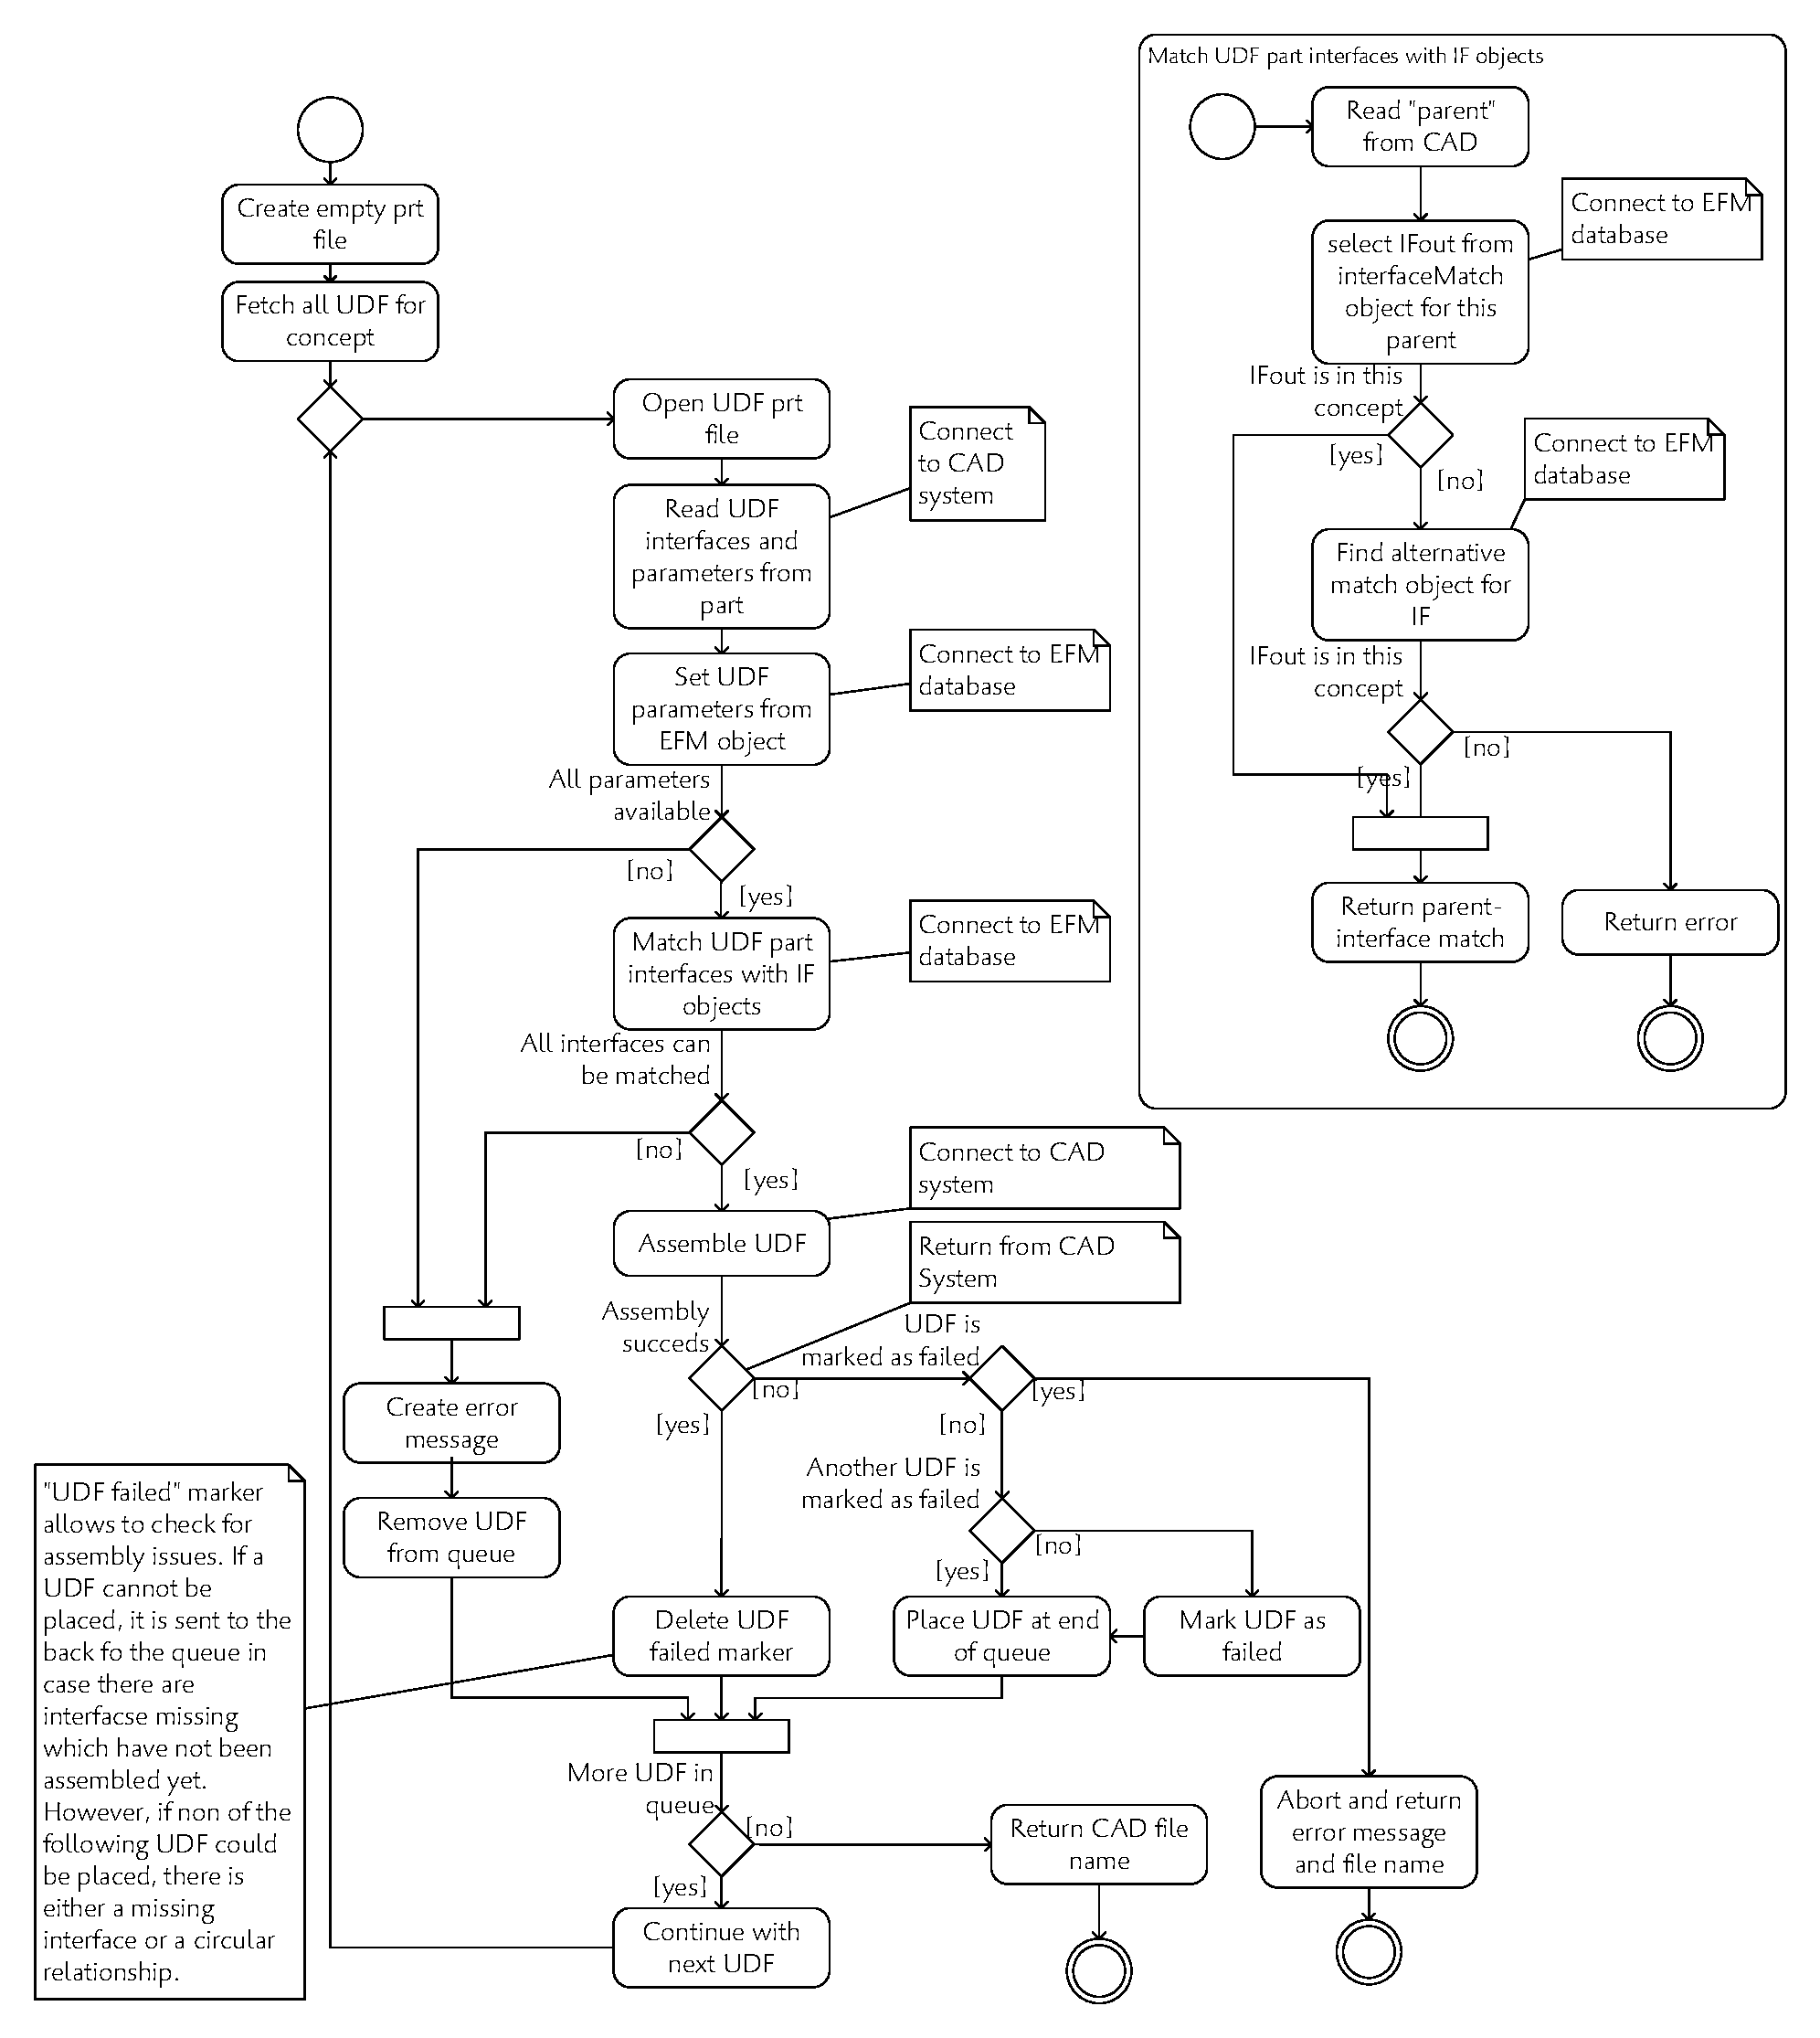
\includegraphics[width=\textwidth]{figures/pdf/assemblyAlgorithm.pdf}
    \caption{UML process model of the assembly algorithm as implemented in the FGE proof of concept tool.}
    \label{fig:assemblyAlgorithm}
\end{figure}
% \unskip
% \subsection{}
% The appendix is an optional section that can contain details and data supplemental to the main text. For example, explanations of experimental details that would disrupt the flow of the main text, but nonetheless remain crucial to understanding and reproducing the research shown; figures of replicates for experiments of which representative data is shown in the main text can be added here if brief, or as Supplementary data. Mathematical proofs of results not central to the paper can be added as an appendix.

% \section{}
% All appendix sections must be cited in the main text. In the appendixes, Figures, Tables, etc. should be labeled starting with `A', e.g., Figure A1, Figure A2, etc. 

%%%%%%%%%%%%%%%%%%%%%%%%%%%%%%%%%%%%%%%%%%
% Citations and References in Supplementary files are permitted provided that they also appear in the reference list here. 

%=====================================
% References, variant A: internal bibliography
%=====================================
\reftitle{References}
% \begin{thebibliography}{999}
% % Reference 1
% \bibitem[Author1(year)]{ref-journal}
% Author1, T. The title of the cited article. {\em Journal Abbreviation} {\bf 2008}, {\em 10}, 142--149.
% % Reference 2
% \bibitem[Author2(year)]{ref-book}
% Author2, L. The title of the cited contribution. In {\em The Book Title}; Editor1, F., Editor2, A., Eds.; Publishing House: City, Country, 2007; pp. 32--58.
% \end{thebibliography}

% The following MDPI journals use author-date citation: Arts, Econometrics, Economies, Genealogy, Humanities, IJFS, JRFM, Laws, Religions, Risks, Social Sciences. For those journals, please follow the formatting guidelines on http://www.mdpi.com/authors/references
% To cite two works by the same author: \citeauthor{ref-journal-1a} (\citeyear{ref-journal-1a}, \citeyear{ref-journal-1b}). This produces: Whittaker (1967, 1975)
% To cite two works by the same author with specific pages: \citeauthor{ref-journal-3a} (\citeyear{ref-journal-3a}, p. 328; \citeyear{ref-journal-3b}, p.475). This produces: Wong (1999, p. 328; 2000, p. 475)

%=====================================
% References, variant B: external bibliography
%=====================================
\externalbibliography{yes}
\bibliography{references}

%%%%%%%%%%%%%%%%%%%%%%%%%%%%%%%%%%%%%%%%%%
%% optional
%\sampleavailability{Samples of the compounds ...... are available from the authors.}

%% for journal Sci
%\reviewreports{\\
%Reviewer 1 comments and authors’ response\\
%Reviewer 2 comments and authors’ response\\
%Reviewer 3 comments and authors’ response
%}

%%%%%%%%%%%%%%%%%%%%%%%%%%%%%%%%%%%%%%%%%%
\end{document}

